% Build: tectonic --outdir ../../../outputs/weyl_note note.tex   (pdfLaTeX also works)
% Figure: python make_figure.py   (reads the committed benchmark summary)
\documentclass[11pt,a4paper]{article}
\usepackage{iftex}
\ifPDFTeX
  \usepackage[T1]{fontenc}
  \usepackage[utf8]{inputenc}
  \usepackage{lmodern}
\fi
\usepackage[margin=24mm]{geometry}
\usepackage{amsmath,amssymb,booktabs,graphicx,microtype}
\usepackage[colorlinks=true,allcolors=blue]{hyperref}
\usepackage{caption}
\captionsetup{font=small,labelfont=bf,labelsep=space}
\captionsetup[figure]{name=Fig.}
\newcommand{\dd}{\mathrm d}
\newcommand{\IB}{Ibrahim and Bombelli}
\newcommand{\doi}[1]{\url{https://doi.org/#1}}
\title{Vacuum tidal curvature from causal order and interval counts:\\
a finite-density estimator and a gravitational-wave benchmark}
\author{Juneyoung Kim\thanks{Corresponding author. E-mail: \texttt{lpaiu.cs@gmail.com}}\\
\small Independent researcher, Seoul, Republic of Korea}
\date{}
\begin{document}
\maketitle
\begin{abstract}
Recent work proves that the Riemann tensor can be reconstructed from the
causal order and element counts of a sprinkled causal set (Madsen,
arXiv:2610.36695) and estimates that detecting one Weyl component of a
plane gravitational wave by discrete geodesic deviation requires
$10^8$--$10^9$ elements (Ibrahim and Bombelli, arXiv:2611.09056). We present
an estimator of the vacuum Weyl tensor from order relations alone and test
its accuracy, uncertainty and cost at finite density. From the relations
between about a hundred landmarks and $N$ events sprinkled in an Alexandrov
interval it fits all ten components, with curvature gradients, the
landmarks' normal coordinates and a covariance that accounts for shared
events. In pre-specified tests on exact vacuum plane waves, (i) nominal
95\% confidence balls contained the true tensor in 509 of 512 cases; (ii)
at tidal norm $0.5$, six cases gave errors of 3.5--7.4\% and error plus
confidence radius of 11.9--18.8\% for $N=2.6$--$7.2\times10^7$; and (iii)
the five-times weaker wave of Ibrahim and Bombelli was detected at
$N=1.7\times10^7$, a density two to four orders of magnitude below their
estimate, but not at $N\le4.2\times10^6$. (iv) Unchanged, it detected the
static tidal field of a Schwarzschild interval of similar strength at
$N=4.2\times10^6$. Detection is not accuracy: for the wave the local model
underestimates the crest curvature by 12\%, which the fit residuals do not
reveal. An appendix proves a conditional, asymptotic convergence statement.
The tests cover plane waves and one Schwarzschild interval, assume vacuum,
and rely on nominal Gaussian uncertainties.
\end{abstract}

\noindent\textbf{Keywords} Causal sets $\cdot$ Weyl tensor $\cdot$ Curvature
estimation $\cdot$ Plane gravitational waves $\cdot$ Schwarzschild spacetime
$\cdot$ Poisson sprinkling

\section{Introduction}
In causal set theory a Lorentzian geometry is to be recovered from a locally
finite partial order together with counting: the order carries the conformal
structure \cite{zeeman,hkm,malament} and the number of elements the volume
\cite{blms,surya,braun}. For sprinklings, that is, Poisson samples of a
spacetime with their induced order, order-only estimators are known for
proper time \cite{myrheim,brightwell}, dimension \cite{myrheim,meyer},
scalar curvature \cite{benincasa}, the Ricci terms that enter the volume of
small intervals \cite{gibbons,roy}, and spatial distance
\cite{rideout,eichhorn,boguna}. Numerical studies of curvature estimators on
sprinkled causal sets have addressed Ricci-type quantities
\cite{kambor,barton}. In vacuum these quantities vanish, and the curvature
that remains is tidal: the ten components of the Weyl tensor.

Several recent works bear on this problem. Madsen~\cite{madsen} constructs
approximate normal coordinates, parallel transport and the full Riemann
tensor from the order and element counts, given the dimension $d$ and the
density $\rho$, and proves a uniform error bound
$C[\log(e+\rho)/\rho]^{1/[2(3d+4)]}$, that is, an exponent of $1/32$ for
$d=4$. That paper contains no numerical experiment, and its conclusion calls
for sharper rates, practical anchor selection and numerical studies of the
error at finite density. \IB~\cite{ib} study geodesic deviation between
geodesic analogs, built from longest maximal chains, in a linearized plane
wave. From the measured thickness of these chains they estimate that
detecting one Weyl component requires $N_{\rm total}\sim10^8$ elements under
their most liberal assumptions and $\sim10^9$ under those they expect, even
with an ideal distance estimator, whereas $3$--$4\times10^6$ elements can be
simulated with their method. Their outlook names the use of more information
from the sprinkling, exact pp-waves and lower memory requirements as next
steps. Shuman~\cite{shumana,shumanb} constructs coordinates, derivatives and
tangent spaces on causal sets, with numerical tests in flat $1+1$
dimensions. In a preprint, Alfyorov and Shnyukov~\cite{alfyorov} propose a
statistic of the Hasse diagram that responds to the scalar invariant
$E_{ij}E^{ij}$ and report simulations of sprinkled pp-wave diamonds with up
to $1.5\times10^4$ elements. Ghosh~\cite{ghosh} discusses bounds on the
number of elements needed to estimate curvature from a finite causal set. In
the continuum, gravitational compasses determine all curvature components
from the relative acceleration of test bodies~\cite{szekeres} or from
comparisons of clocks~\cite{puetzfeld}.

This paper presents an estimator of the Weyl tensor that was applied to
sprinkled data, together with measurements of its accuracy, coverage and
cost. It makes four limited claims. First, on exact vacuum plane waves all
ten components were estimated from order relations alone, with tested
accuracy, at event counts that a single workstation can handle. Second, the
uncertainty reported by the estimator was tested for coverage on a stated
population of cases. Third, at the condition analysed in Ref.~\cite{ib} the
estimator detected the wave. Fourth, without any change it detected the
tidal field of a Schwarzschild exterior, which is static and of a different
algebraic type. We do not claim the first reconstruction of curvature from
a causal set, an unconditional convergence theorem, or greater efficiency
than another method applied to the same input. Section~\ref{setting} defines
the setting and the estimand, Sect.~\ref{estimator} the estimator and
Sect.~\ref{tests} the tests; Sect.~\ref{results} reports the results and
Sect.~\ref{limits} the limitations. Appendix~\ref{app:conv} proves a
conditional convergence statement for the fit.

\section{Setting and estimand}\label{setting}
Let $(M,g)$ be a four-dimensional Ricci-flat spacetime and $p\prec q$ two
events whose Alexandrov interval $I(p,q)=J^+(p)\cap J^-(q)$ lies in a convex
normal neighbourhood. Let $T$ be the proper time from $p$ to $q$. Sprinkle
$N$ events independently and uniformly with respect to volume in $I(p,q)$,
that is, a Poisson sprinkling conditioned on its number of events. The data
are order relations among the sprinkled events and the two tips. No
coordinates, metric functions, density or flat reference sample are given.

Two exact invariances bound what can be estimated. Under
$g\to\lambda^2g$ the order and the sampling law are unchanged while
orthonormal curvature components scale as $\lambda^{-2}$, so only
$T^2C_{abcd}$ is identifiable. A spatial reflection also preserves the
order, so the tensor is determined at most up to parity. The estimand is
therefore $T^2C_{abcd}$ at the midpoint of the tip geodesic, in an
orthonormal frame whose time axis is the tip direction and whose spatial
axes are fixed by two landmarks, modulo one reflection. Equivalently it is
the pair $E_{ij}=C_{0i0j}$, $B_{ij}=\tfrac12\epsilon_{ikl}C_{kl0j}$. We
measure size and error by the full tidal norm
$s=T^2(E_{ij}E_{ij}+B_{ij}B_{ij})^{1/2}$.

\section{Estimator}\label{estimator}
\subsection{Interval clocks}
For $x\prec y$ in $I(p,q)$ let $n(x,y)$ be the number of sprinkled events in
$I(x,y)$. Every event lies in $I(p,q)$, so $n(x,y)/N$ estimates
$V(x,y)/V(p,q)$ without bias. In vacuum a small interval has
$V=(\pi/24)\tau^4[1+O(C^2\tau^4)]$, because the $O(\tau^2)$ correction is
built from the Ricci tensor \cite{gibbons,roy}. Hence
\begin{equation}
 y(x,y)=-\sqrt{n(x,y)/N} \label{clock}
\end{equation}
estimates the signed squared interval $\sigma(x,y)=-\tau(x,y)^2/T^2$ up to
curvature-squared terms, with no reference to the density. One event belongs
to many intervals, so the clocks are strongly correlated. For intervals $a$
and $b$,
\begin{equation}
 \operatorname{Cov}\!\left(n_a/N,\,n_b/N\right)=(\pi_{ab}-\pi_a\pi_b)/N,
 \label{cov}
\end{equation}
where $\pi_a$ is the probability of $I_a$ and $\pi_{ab}$ that of
$I_a\cap I_b$. We estimate \eqref{cov} from the exact empirical frequencies
of joint membership and propagate it to \eqref{clock} by the delta method,
which gives the clock covariance $\widehat\Sigma$.

\subsection{Model}
Give each landmark normal coordinates $x_i\in\mathbb R^4$ based at the
midpoint of the tip geodesic, in units of $T$, with the tips at
$(\mp\tfrac12,0,0,0)$. Write $\Delta=x-y$, $\eta=\operatorname{diag}(-1,1,1,1)$
and $C(x,y,x,y)=C_{abcd}x^ay^bx^cy^d$. The world-function expansion
\cite{brewin} gives
\begin{equation}
 \sigma(x,y)=\eta(\Delta,\Delta)-\tfrac13C(x,y,x,y)
 -\tfrac1{12}(x+y)^e\nabla_eC(x,y,x,y)+\sigma_2(x,y;C)+\cdots,
 \label{model}
\end{equation}
with all tensors at the origin. The omitted terms start with second
covariant derivatives of the curvature. The term $\sigma_2$ collects the
known curvature-squared contributions and has no free parameter:
\begin{align}
 \sigma_2&=\tfrac1{45}\left(4\,u\!\cdot\!v-u\!\cdot\!u-v\!\cdot\!v\right)
 +\tfrac12\eta(\Delta,\Delta)\left[\kappa(\Delta)-\kappa(\Delta_0)\right],\nonumber\\
 \kappa(\Delta)&=\frac{20\,E_{ab}(\Delta)E^{ab}(\Delta)-3\,\eta(\Delta,\Delta)^2K}{10080},
 \qquad E_{ab}(\Delta)=C_{acbd}\Delta^c\Delta^d,\quad
 K=\tfrac18C_{abcd}C^{abcd}. \label{square}
\end{align}
Here $u_a=C(x,y,x,e_a)$, $v_a=C(x,y,y,e_a)$ and dots are taken with $\eta$.
The first part is the second-order world function \cite{brewin}. The second
converts volume clocks to proper times for both the interval and the
reference interval, whose separation is $\Delta_0=(1,0,0,0)$; it uses the
vacuum expansion $V=(\pi/24)\tau^4[1+\kappa+\cdots]$, where
$\kappa=\tau^4(17E^2+3B^2)/10080$ for the observer along
$\Delta$.\footnote{This coefficient was derived independently and checked
against exact plane-wave volumes: with it, the residual of the volume clock
for a constant wave with $s=1.5$ falls from $3.9\times10^{-4}$ to
$1.7\times10^{-6}$. A plane wave has $E^2=B^2$ and tests only the sum of
the two coefficients. For the Schwarzschild interval of Sect.~\ref{tests},
where $B=0$, a quadrature of the volume gives an excess over
$(\pi/24)\tau^4$ of $1.0004$ times $17E^2\tau^4/10080$ at $r_a=6M$,
$\tau=M/2$, and of $1.015$ times that value at $\tau=3M$. We were unable to
reproduce the corresponding
coefficient of Eq.~(79) in Ref.~\cite{wang} (arXiv version 2), from which
ours differs by about 15\% for a plane wave. The term $\sigma_2$ changes the
fitted curvature by about 1\% at $s=1.5$ and by less at weaker curvature.}

The unknowns are the landmark coordinates, the ten Weyl components $c$ in a
fixed basis of five electric and five magnetic tensors, and the 24
components $g$ of $\nabla C$ allowed by the vacuum Bianchi identity. The
rotation gauge is fixed by placing the first landmark in the $(t,x)$ plane
and the second in the $(t,x,y)$ hyperplane, which leaves $4L-3$ coordinates
for $L$ landmarks. No algebraic type, polarization or profile is imposed.

\subsection{Linear response and identifiability}
With normal coordinates based at an event $o$, the quantity
$G_{xy}=\tfrac12(\sigma_{ox}+\sigma_{oy}-\sigma_{xy})
=\eta(x,y)+\tfrac16C(x,y,x,y)+\cdots$ is a Gram matrix in flat spacetime.
For four reference events $a_i$ with Gram matrix $G_A$ and
$g_x=(G_{a_ix})$, flat geometry forces the Schur residual
$D_{xy}=G_{xy}-g_x^{\!\top}G_A^{-1}g_y$ to vanish. To first order in the
curvature, with $k_x=G_A^{-1}g_x$,
\begin{equation}
 6D_{xy}=C(x,y,x,y)-\sum_ik_{yi}C(a_i,x,a_i,x)-\sum_ik_{xi}C(a_i,y,a_i,y)
 +\sum_{ij}k_{xi}k_{yj}C(a_i,a_j,a_i,a_j). \label{schur}
\end{equation}
The failure of interval data to embed in flat spacetime is thus linear in
$C$. Lorentzian Gram embedding is established~\cite{clough} and is also the
coordinate step of Ref.~\cite{madsen}; the residual \eqref{schur} is what
carries the tidal information. The estimator does not solve \eqref{schur};
it fits \eqref{model} jointly, so that every clock and its covariance are
used. Exact rational computations for explicit timelike configurations give
the response matrix of \eqref{schur} rank ten, and rank 34 when the gradient
terms of \eqref{model} are added. Nonvanishing minors are polynomial
statements, so all 34 parameters are generically locally identifiable. This
says nothing about conditioning. In particular, if every landmark lies on
one of two time slices, write $x=(t,\mathbf r)$, $y=(s,\mathbf z)$ and
$\mathbf F(\mathbf r)=\mathbf r\times(B\mathbf r)$; the magnetic part of the
response is $2[t\,\mathbf r\!\cdot\!\mathbf F(\mathbf z)
+s\,\mathbf z\!\cdot\!\mathbf F(\mathbf r)]$, and the displacements
$\delta\mathbf r=s\mathbf F(\mathbf r)/3$,
$\delta\mathbf z=t\mathbf F(\mathbf z)/3$ reproduce its effect on every
cross-slice interval while leaving the clocks to the tips unchanged. All
five magnetic components are then absorbed by the unknown positions at first
order. A third time band removes the degeneracy, which is why the landmarks
are placed in three bands.

\subsection{Landmark selection}
Landmarks are chosen from the order of an independent selection sample of
4096 events, so that the selection does not condition the measurement
sample. For candidate $i$ the counts to the tips give
$\alpha_i=\sqrt{n_{pi}/n_{pq}}$ and $\beta_i=\sqrt{n_{iq}/n_{pq}}$, and the
flat proxies $t_i=(\alpha_i-\beta_i)/2$,
$r_i^2=\tfrac14+t_i^2-(\alpha_i+\beta_i)/2$. Candidates are kept in three
bands, $t\in[-0.36,-0.24]$, $|t|\le0.075$ and $t\in[0.24,0.36]$, with
$0.075\le r\le0.2$. They are ranked by connectivity and radius and pruned
until every landmark has at least eight clocks and every central landmark
at least four to each outer band. We use the union of the selections with
caps of 64 and 128 landmarks. In the accuracy test, the benchmark and the
Schwarzschild test below this gave 104--131 landmarks and
$2.8$--$4.5\times10^3$ clocks, a clock
being a related pair whose interval holds at least two selection events.
These settings were fixed in preliminary runs before the tests reported
here. The estimator then needs, for each measurement event, only its
relations to the landmarks: $2LN$ bits, and no $N\times N$ order matrix.

\subsection{Fit and uncertainty}
The estimate minimizes
$\chi^2(\theta)=[y-\sigma(\theta)]^{\!\top}\widehat\Sigma^{-1}[y-\sigma(\theta)]$
over $\theta=(x_i,c,g)$ by Levenberg--Marquardt iteration from four
deterministic starts built from the tip clocks. The covariance $S$ of
$\hat c$ is the corresponding block of $(J^{\!\top}\widehat\Sigma^{-1}J)^{-1}$,
with $J$ the Jacobian at the solution. We report the ball
\begin{equation}
 \|C-\widehat C\|\le r=\frac{(\chi^2_{10;\gamma}\,\lambda_{\max})^{1/2}
 +\delta\|\widehat C\|}{1-\delta}, \label{ball}
\end{equation}
where $\lambda_{\max}$ is the largest eigenvalue of $S$ in the tidal metric,
$\gamma$ the nominal coverage and $\delta=0.02$ an allowance for model bias.
The allowance is an assumption that the tests check; it is not derived from
the data. For detection we use $Q=\hat c^{\top}S^{-1}\hat c$, nominally
$\chi^2_{10}$ in flat spacetime.

\section{Numerical tests}\label{tests}
\subsection{Test geometries}
The tests use exact vacuum plane waves in Brinkmann form,
\begin{equation}
 \dd s^2=2\,\dd u\,\dd v+H_{ab}(u)x^ax^b\,\dd u^2+\delta_{ab}\dd x^a\dd x^b,
 \qquad\operatorname{tr}H=0, \label{wave}
\end{equation}
with tips $p=(u,v,x)=(0,\tfrac12,0)$ and $q=(1,-\tfrac12,0)$. Then
$T=\sqrt2$, $R_{uaub}=-H_{ab}$, and the midpoint tidal norm is $s=2A$ when
$H(\tfrac12)$ has eigenvalues $\pm A$. Two families are used: a rotating
polarization, $H(u)=R_\phi\operatorname{diag}(A,-A)R_\phi^{\!\top}$ with
$\phi=w(u-\tfrac12)$, $A\in\{0,0.25,0.75\}$ and $w\in\{0,\pm0.5\}$; and the
oscillating profile of Sect.~\ref{ibwave}. Since $\det g=-1$, uniform
sampling in the chart is uniform in volume. Two events with $u_x<u_y$ are
related exactly when $v_x-v_y$ exceeds the minimal transverse action between
them, a quadratic form in the transverse endpoints built from the Jacobi
propagator~\cite{harte}. The generators evaluate it with guarded
floating-point margins and never guess a pair inside the guard.

One further test uses the Schwarzschild exterior in isotropic coordinates,
\begin{equation}
 \dd s^2=-\left(\frac{2\bar r-M}{2\bar r+M}\right)^{\!2}\dd t^2
 +\left(1+\frac{M}{2\bar r}\right)^{\!4}\delta_{ij}\dd X^i\dd X^j,
 \qquad\bar r=|X|. \label{schw}
\end{equation}
The tips lie on the radial geodesic that is momentarily at rest at areal
radius $r_a$, at proper times $\mp T/2$ from this apex, which is therefore
the midpoint of the tip geodesic. In the rest frame of that geodesic at the
apex, with the radial axis first,
$T^2E=(T^2M/r_a^3)\operatorname{diag}(-2,1,1)$ and $B=0$, so that
$s=\sqrt6\,T^2M/r_a^3$. Because the metric is static, two events are related
exactly when their difference in $t$ is at least the optical distance
between their spatial positions, the minimum over paths of
$\int(1+M/2\bar r)^3(1-M/2\bar r)^{-1}|\dd X|$. The generator finds this
minimum by Newton iteration on a polynomial deviation from the straight
chord and samples uniformly with respect to
$\sqrt{-g}=(1-M/2\bar r)(1+M/2\bar r)^5$. Its travel times
agree with the exact radial formula and with an independent solver that uses
the Clairaut constant in areal coordinates; the tidal tensor was confirmed
by integrating the geodesic deviation, and the sampling measure by a
quadrature of the volume. Flat controls for this test come from the same
generator with $M=0$.

\subsection{Blind estimation and pre-specified criteria}\label{procedure}
The estimator runs in a separate process that reads only an order archive
containing the selection order, the landmark labels, the landmark--event
relation bits and $N$. The generator and the true geometry are accessed only
after the fit has been written to disk. For each test, the cases, random
seeds, sample sizes, statistics, thresholds and rules for failed cases were
fixed and recorded in a version-controlled repository before the
corresponding data were generated. No case was regenerated, extended or
removed, and failed cases are counted as failures. Two quantities use the
true geometry: the error $\|\widehat C-C\|$, taken modulo the reflection,
and the \emph{continuum bias}, obtained by applying the same fit to exact
interval volumes on the same landmarks, which isolates the error of the
model \eqref{model}. After each test, separately written code recomputed all
reported outcomes from the saved fits.

\subsection{Implementation and use of AI tools}\label{implementation}
The estimator, the generators and the checking code are written in Python
with NumPy~\cite{numpy} and SciPy~\cite{scipy}. The relation tests and the
integer sums of the clock covariance were run on a graphics processor with
the CuPy library. All runs used one workstation with eight CPU cores,
126\,GiB of memory and one graphics processor.

Large language models (OpenAI Codex and Anthropic Claude) were used
extensively in this work, under the direction of the author: for writing and
running the code, for the derivations and proofs and their numerical
checks, for the comparison with the literature and for drafting the text.
Since such tools can produce plausible errors, the numerical conclusions
rest on the safeguards of Sect.~\ref{procedure}: criteria fixed before the
data were generated, an estimator isolated from the true geometry, no
exclusion of cases, and recomputation of the outcomes by separate code. The
proofs of Appendix~\ref{app:conv} were rederived line by line in a separate
pass, and the orders they assert were checked numerically
(Sect.~\ref{app:check}). The bibliographic data of
all references were checked against publisher, arXiv or repository records. The author
has examined the results and the text and takes full responsibility for
them.

\section{Results}\label{results}
\subsection{Coverage}
We generated 512 independent cases from the product mixture
$A\in\{0,0.25,0.75\}$, $w\in\{0,\pm0.5\}$, each with $N=262{,}144$. A case
counts as a success if the fit is valid, its continuum bias is at most 2\%,
and the true tensor lies in the ball \eqref{ball} with $\gamma=0.95$. There
were 509 successes, which gives an exact two-sided 95\% confidence interval
\cite{clopper} of $[0.983,0.999]$ for the success probability; the
pre-specified requirement was a lower limit of at least $0.95$. Two of the
failures had an empty measurement clock, and in one flat case the ball did
not contain the true tensor. At this $N$ the balls are wide, so this test
concerns the reliability of the reported uncertainty and not precision. An
earlier version of the estimator, without $\sigma_2$, did not meet the same
requirement: it had 246 successes in 256 cases, and nine of the failures
were violations of the bias allowance. We report that result unchanged; it
is the reason for including $\sigma_2$.

\subsection{Accuracy at weak curvature}
The pre-specified criterion required, jointly for eight cases, a continuum
bias of at most 2\%, the true tensor inside the ball, and an error plus
radius of at most 25\% of $s$ for six cases with $A=0.25$ ($s=0.5$), or at
most $0.125$ for two flat cases. The family confidence level was 95\%, so
that each ball has $\gamma=0.99375$, and the sample sizes were chosen for
90\% joint power from bounds on $N\lambda_{\max}$ fixed in advance. All
eight cases met the criterion (Table~\ref{accuracy}). The two flat cases had
errors of $0.023$ and $0.022$ with radii of $0.056$. For the three landmark
selections that had been used in an earlier diagnostic run,
$N\lambda_{\max}$ changed by less than 0.5\% between $N=4.2\times10^6$ and
the final $N$, so the noise decreases as $N^{-1/2}$. The number of events
needed for a given relative precision is therefore proportional to
$N\lambda_{\max}/s^2$; $N\lambda_{\max}$ was between $2.2\times10^3$ and
$6.7\times10^3$ for the selections of this test and of the diagnostic run,
between $2.6\times10^3$ and $3.5\times10^3$ in the benchmark below, and
between $2.6\times10^3$ and $4.4\times10^3$ in the Schwarzschild test. In
the diagnostic run, which had no pre-specified accuracy criterion, the
stronger waves with $A=0.75$ gave errors of 1.6--5.9\% at
$N=4.2\times10^6$.

\begin{table}[t]
\centering\small
\caption{Weak-curvature accuracy test, $s=0.5$. Errors, radii and biases
are percentages of the true tidal norm; the radius is that of the
simultaneous ball of Eq.~\eqref{ball} with $\gamma=0.99375$}
\label{accuracy}
\begin{tabular}{rrrrrrr}
\toprule
Case & $w$ & $N/10^6$ & Error & Radius & Error $+$ radius & Continuum bias\\
\midrule
2 & $0$ & 49.3 & 3.85 & 11.59 & 15.44 & 0.004\\
3 & $+0.5$ & 51.1 & 7.36 & 11.47 & 18.83 & 1.24\\
4 & $-0.5$ & 26.0 & 5.03 & 11.39 & 16.42 & 1.28\\
5 & $-0.5$ & 71.7 & 3.46 & 8.47 & 11.94 & 1.25\\
6 & $0$ & 71.7 & 5.20 & 11.85 & 17.05 & 0.003\\
7 & $+0.5$ & 71.7 & 4.48 & 8.98 & 13.45 & 1.26\\
\bottomrule
\end{tabular}
\end{table}

\subsection{The wave of \IB}\label{ibwave}
The linearized wave of Ref.~\cite{ib} has amplitude $h_0=10^{-2}$ and tidal
profile $\tfrac12\omega^2h_0\cos[\omega(t-z)]$ along the central observer,
in a region of height $H=\lambda/2$ with a crest at mid-height. In the units
of \eqref{wave} this is $\omega T=\pi$ and
\begin{equation}
 H(u)=A_0\sin(\pi u)\operatorname{diag}(1,-1),\qquad
 A_0=\pi^2h_0/2=0.0493,\qquad s=2A_0=0.0987 .
\end{equation}
The wave is five times weaker than in Table~\ref{accuracy} and varies by
half a cycle across the window. We use the exact vacuum wave with this axis
profile, since the linearized metric is vacuum only to first order in $h_0$;
the polarization is rotated by a quarter turn, which the estimator does not
use. The estimator, the landmark rule and the uncertainty were not changed.

The criterion was fixed before the data were generated. At each of four
nested levels $N=2^{20},2^{22},2^{24},2^{26}$, with two independent wave
cases and two independent flat controls, the level counts as a detection if
$Q>q^*=\chi^2_{10}(0.999)=29.59$ in both wave cases and in neither control.
Table~\ref{benchmark} and Fig.~\ref{fig} give the outcome: no detection at
$1.05\times10^6$ events, a mixed outcome at $4.19\times10^6$, and detection
at $1.68\times10^7$ and $6.71\times10^7$. The eight control values average
$11.2$, consistent with the $\chi^2_{10}$ mean of 10, but two independent
controls cannot test a $10^{-3}$ tail, so the false-positive level is
nominal. The predictions recorded with the criterion were
$Q\approx15,33,100,370$ and a continuum bias of 10--20\%.

\begin{table}[t]
\centering\small
\caption{Detection statistic $Q$ at the condition of Ref.~\cite{ib};
threshold $q^*=29.59$. Levels are nested prefixes of one event stream per
case, so the rows are not independent}
\label{benchmark}
\begin{tabular}{rrrrrl}
\toprule
$N$ & Wave 0 & Wave 1 & Flat 2 & Flat 3 & Outcome\\
\midrule
1,048,576 & 11.02 & 15.70 & 10.62 & 4.36 & not detected\\
4,194,304 & 16.24 & 29.98 & 17.78 & 9.84 & mixed\\
16,777,216 & 75.60 & 97.03 & 11.46 & 10.87 & detected\\
67,108,864 & 347.12 & 313.70 & 10.82 & 13.47 & detected\\
\bottomrule
\end{tabular}
\end{table}

\begin{figure}[t]
\centering
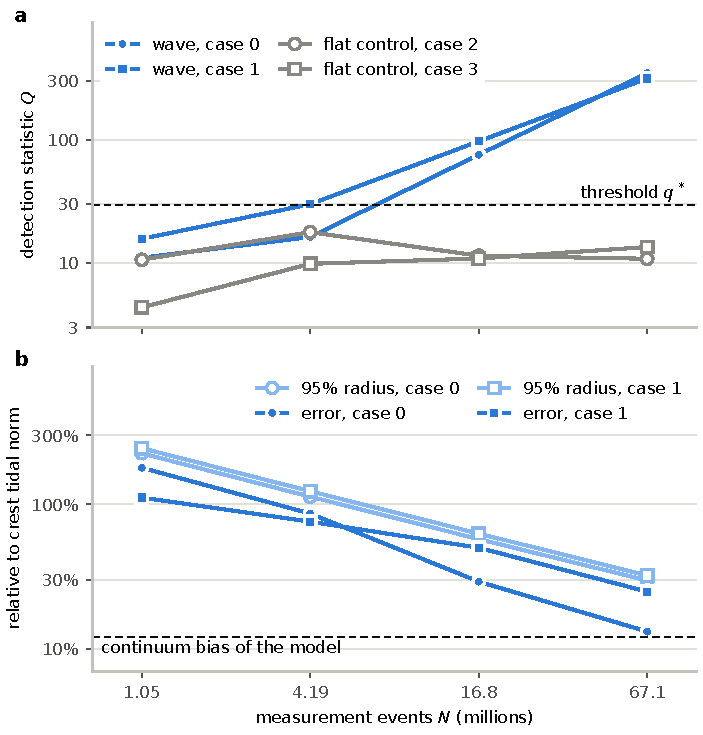
\includegraphics[width=119mm]{Fig1.pdf}
\caption{Benchmark at the condition of Ref.~\cite{ib}. \textbf{a} Detection
statistic $Q$ for the two wave cases (filled symbols) and the two flat
controls (open symbols); circles and squares mark the independent cases of
each kind, and the dashed line is the threshold $q^*=29.59$. \textbf{b}
Full-tidal error (filled symbols) and nominal 95\% confidence radius (open
symbols) of the two wave cases, relative to the crest tidal norm; the dashed
line is the bias of the model in the continuum limit}
\label{fig}
\end{figure}

This result is a detection and not an accurate measurement. At the top
level the errors are 13\% and 25\% of $s$, with nominal 95\% radii of 30\%
and 32\%. The estimated electric eigenvalues, $(-0.0455,0.0003,0.0451)$ and
$(-0.0429,0.0026,0.0403)$, show the pattern of the true ones,
$(-0.0493,0,0.0493)$. The continuum bias is 12.1\% and 11.6\%: the fit
returns a window-averaged curvature, $0.88$--$0.89$ of the crest value,
because the half-cycle variation lies outside \eqref{model}. This violates
the allowance $\delta$, so the balls are not accuracy statements for this
wave. The residuals do not show the misfit: the continuum refit has
$\chi^2\approx0.3$ at the top level, and the sixteen finite fits have
$\chi^2$ within $2.3$ standard deviations of their
$3.1$--$3.9\times10^3$ degrees of freedom. The nominal signal-to-noise ratio
along the electric pattern of the true tensor reaches one at
$N=2.6$--$2.8\times10^5$.

Two further observations are post hoc and were not part of the criterion.
The noncentrality implied by the continuum refit predicts $Q=14$--$15$,
$28$--$29$, $80$--$87$ and $290$--$316$ at the four levels, within $1.4$
standard deviations of all eight observed values, and places 50\% and 90\%
detection power at $N\approx4.5$--$4.9\times10^6$ and
$7.7$--$8.4\times10^6$. Moreover, only about $1.6\times10^{-4}$ of the
landmark--event relations differ from those of the flat metric in the same
chart (86 and 83 of about $5\times10^5$ among the first 4096 events); the
whole signal is carried by these.

\subsection{Comparison in common units}
The number $N_{\rm total}$ of Ref.~\cite{ib} counts elements in a thin box
of volume $(a_w\delta)^2(L+a_w\delta)H$ around two chains of thickness
$\delta/H=A_4(\pi\rho H^4/24)^{-\beta_4}$, with $A_4\approx0.30$--$0.32$ and
$\beta_4\approx0.11$. With their most liberal $a_w=2$ and $L=\lambda/2$,
their Eq.~(20), $N_{\rm total}\approx4.5\times10^{11}/m^{7/2}$, gives the
densities in Table~\ref{units}, where $m$ is the number of mid-level
elements of each chain bundle. Our $N$ counts events in the whole interval
of height $H$, of volume $\pi H^4/24$. The level at which the pre-specified
criterion was met lies at a density $2.4\times10^2$ ($m=11$) to
$2.7\times10^4$ ($m=4$) times lower, or at a discreteness scale
$\ell=\rho^{-1/4}$ that is 4 to 13 times coarser, under a stricter
criterion.

\begin{table}[t]
\centering\small
\caption{Event counts in common units. $H$ is the height of the region and
$\ell=\rho^{-1/4}$. The first two rows are the requirement estimated in
Ref.~\cite{ib} for geodesic deviation with an ideal distance estimator, for
which no recovery was performed; the last three rows are this work. S/N
denotes the signal-to-noise ratio}
\label{units}
\begin{tabular}{@{}llrrr@{}}
\toprule
 & Criterion & Events & $\rho H^4$ & $H/\ell$\\
\midrule
Ref.~\cite{ib}, $m=11$ & S/N $=1$, one component & $1.0\times10^8$ (box) & $3.1$--$3.6\times10^{10}$ & 420--440\\
Ref.~\cite{ib}, $m=4$--$5$ & S/N $=1$, one component & $1.6$--$3.5\times10^9$ (box) & $1.1$--$3.5\times10^{12}$ & 1020--1370\\
\midrule
nominal & S/N $=1$, electric pattern & $2.6$--$2.8\times10^5$ & $2.0$--$2.1\times10^6$ & 38\\
post hoc & $Q>q^*$ with 90\% power & $7.7$--$8.4\times10^6$ & $5.9$--$6.4\times10^7$ & 88--90\\
pre-specified & $Q>q^*$, both waves, no control & $1.68\times10^7$ & $1.28\times10^8$ & 106\\
\bottomrule
\end{tabular}
\end{table}

This is not a like-for-like comparison of two procedures. The number of
Ref.~\cite{ib} is an estimated requirement for measuring the separation of
two chains. Our estimator uses the relations between all events of the
interval and about 130 landmarks, assumes vacuum, and fits a local model.
We did not implement geodesic deviation, and neither method was applied to
the input of the other. The difference is in the direction anticipated in
the outlook of Ref.~\cite{ib}: more information from the sprinkling, an
exact vacuum wave, and lower memory requirements.

\subsection{A Schwarzschild interval}\label{schwres}
The tests above use plane waves, which are of Petrov type N with electric
and magnetic parts of equal norm. To test the estimator outside this class
we applied it, unchanged, to an interval of the metric \eqref{schw} with
$r_a=6M$ and $T=3M$. The true tensor is static, of type D and purely
electric, $T^2E=\operatorname{diag}(-\tfrac1{12},\tfrac1{24},\tfrac1{24})$,
with $s=0.102$, close to the strength of the wave of Sect.~\ref{ibwave}. It
is far from uniform: the interval covers areal radii from $4.8M$ to $7.2M$,
over which $M/r^3$ ranges from $1.93$ to $0.57$ times its value at the apex.
Exact interval volumes were not available for this geometry, so the
continuum bias was not measured, and the errors below include it.

The criterion, the levels and the threshold were those of
Sect.~\ref{ibwave} and were fixed before the data were generated, with two
independent Schwarzschild cases and two flat controls.
Table~\ref{schwtable} gives the outcome: a mixed outcome at $1.05\times10^6$ events, where only one of the two
Schwarzschild cases exceeded the threshold, and detection at
$4.19\times10^6$, $1.68\times10^7$ and $6.71\times10^7$. The eight control
values average $10.2$. The
predictions recorded with the criterion, obtained from the covariances of
the benchmark fits, were $Q\approx19,44,150,560$, with no detection
expected at the lowest level and a detection or a mixed outcome at the
second. The value $32.1$ at the lowest level lies $2.3$ nominal standard
deviations above the expectation for that case, $16.5$; the other seven
values of the Schwarzschild cases lie within $1.3$.

\begin{table}[t]
\centering\small
\caption{Detection statistic $Q$ for the Schwarzschild interval; threshold
$q^*=29.59$. Levels are nested prefixes of one event stream per case, so
the rows are not independent}
\label{schwtable}
\begin{tabular}{rrrrrl}
\toprule
$N$ & Schwarzschild 0 & Schwarzschild 1 & Flat 2 & Flat 3 & Outcome\\
\midrule
1,048,576 & 32.14 & 19.27 & 6.20 & 9.94 & mixed\\
4,194,304 & 42.00 & 42.12 & 10.45 & 9.46 & detected\\
16,777,216 & 140.29 & 158.44 & 10.10 & 13.13 & detected\\
67,108,864 & 462.38 & 534.25 & 10.57 & 11.47 & detected\\
\bottomrule
\end{tabular}
\end{table}

At the top level the errors are 16.5\% and 14.4\% of $s$, with
nominal 95\% radii of 37\% and 34\%, and the balls contain the
true tensor at every level. The estimated electric eigenvalues,
$(-0.0846,0.0390,0.0456)$ and $(-0.0800,0.0382,0.0418)$, show the pattern
of the true ones, $(-0.0833,0.0417,0.0417)$, and the estimated magnetic
parts, which should vanish, have norms $0.016$ and $0.013$, against radii
of $0.038$ and $0.034$. The component of each estimate along the true
tensor, weighted by $S^{-1}$, is $1.05\pm0.05$ and $0.97\pm0.04$ times that
tensor, so no bias is resolved at this precision. The fitted landmark
coordinates agree with the true normal coordinates to an rms of
$10^{-4}\,T$. As in Sect.~\ref{ibwave}, this is a detection of the field
and not an accurate measurement: error plus radius is still about half of
$s$. The nominal signal-to-noise ratio along the true tensor reaches one at
$N=1.2$--$1.7\times10^5$.

One auxiliary run preceded the criterion and is reported for completeness.
To test the software we used a larger interval at the same apex, $T=4M$
with $s=0.18$, which gave $Q=9.2$, $86.5$ and $393.7$ at the first three
levels and read $0.94\pm0.05$ of the true tensor at the third. Its first
$2^{24}$ events, cut into sixteen disjoint blocks of $2^{20}$ and fitted
with the same landmarks, gave a mean $Q$ of $37.0$, where the true tensor
and the nominal covariance imply $37.2$, but a mean of $13.4$ for the
statistic of the estimate about the true tensor, where $10$ is nominal.
At about $10^6$ events the nominal covariance may thus understate the
scatter by some 15\% in standard deviation. This concerns one selection and
was not a pre-specified test.

\subsection{Computational cost}
The accuracy test used $3.9\times10^8$ measurement events and
$9.8\times10^{10}$ landmark--event relation tests, and ran in 50 minutes
with a peak memory of 52\,GiB. The benchmark used $2.7\times10^8$ events and
$7.0\times10^{10}$ relation tests, and ran in 60 minutes with a peak of
55\,GiB. At the level of detection one fit takes about three minutes and
13--34\,GiB. The Schwarzschild test used $2.7\times10^8$ events and
$6.8\times10^{10}$ relation tests, and ran in 74 minutes with a peak of
52\,GiB.

\section{Limitations and outlook}\label{limits}
The first limitation is that detection is not accuracy. The bias of the
model was at most 0.004\% for constant profiles, 1.2--1.3\% for $|w|=0.5$,
and 12\% for the half-cycle wave, and the order data alone did not reveal
it. An accuracy statement therefore needs a regularity assumption on how the
curvature varies across the window. Such an assumption cannot be avoided.
For $H_w(u)=a\cos[w(u-\tfrac12)]\operatorname{diag}(1,-1)$ with fixed $a$,
an integration by parts along the minimizing path bounds the difference
between the minimal transverse action and its flat value by a constant times
$aR^2/w$ for transverse endpoints bounded by $R$. For any fixed $N$ the
probability law of the sampled order~\cite{bombelli} thus approaches that of
flat spacetime as $w\to\infty$, while the midpoint tidal norm stays $2a$, so
no estimator is uniformly accurate over all smooth vacuum profiles at fixed
$N$.

The second limitation is scope. The tests cover plane waves and one
Schwarzschild interval. No algebraic type is imposed, but a field with
independent electric and magnetic parts, such as that of a rotating source,
was not tested, and neither was a second radius or interval size. The
estimator assumes vacuum, because Ricci terms enter \eqref{clock} and
\eqref{model} at lower order; it also assumes uniform sprinkling, a regular
normal neighbourhood and given tips. Its uncertainty is nominal and
Gaussian. Coverage was tested at $N=2.6\times10^5$ on one population; at
larger $N$ it rests on the cases reported above and on six flat controls,
and the block test of Sect.~\ref{schwres} suggests that the nominal
covariance is somewhat too small at $N\approx10^6$.

Third, what we can prove about convergence is conditional and asymptotic.
At a fixed window the noise decreases as $N^{-1/2}$ and the bias is fixed by
the window. Appendix~\ref{app:conv} shows that, for a well-conditioned
configuration of landmarks, the solution of the fit near the true geometry
satisfies $\hat c/T^2-C=O(T^2)+O_p(\rho^{-1/2}T^{-4})$ as the window
shrinks at sprinkling density $\rho$, which gives the rate $\rho^{-1/6}$
for $T\propto\rho^{-1/12}$. It does not show that the landmark rule
produces such configurations or that the optimizer finds that solution, it
says nothing about coverage, and its constants are far too conservative to
reach the event counts of the tests. Unlike the theorem of
Ref.~\cite{madsen}, it is restricted to vacuum, to given tips and to one
point. A proof for the implemented procedure, tests on further vacuum
geometries, and a comparison with geodesic deviation on equal inputs are
the natural next steps.

\appendix
% appendix_convergence.tex: fragment for \appendix% appendix_convergence.tex: fragment for \appendix% appendix_convergence.tex: fragment for \appendix\input{appendix_convergence} in note.tex.
% Packages: amsmath and amssymb only (already loaded by note.tex); no amsthm.
% Labels of note.tex used: setting, estimator, tests, limits, clock, cov, model, square, ball.
% Citation keys used: brewin, gibbons, wang, madsen, and ONE new key, oneill:
%   \bibitem{oneill} O'Neill, B.: Semi-Riemannian Geometry with Applications to
%   Relativity. Academic Press, New York (1983)
% Check of the orders and of the rank certificate: python check_convergence_orders.py
\section{A conditional convergence statement}\label{app:conv}
This appendix states what we can prove about the fit of
Sect.~\ref{estimator} in shrinking windows, and what we cannot. The
statement is conditional: it assumes that the landmarks form a
well-conditioned configuration, and it concerns the solution of the fit that
lies near the true geometry. It does not show that the selection rule and
the optimizer of Sect.~\ref{estimator} meet these two conditions, and it
says nothing about the coverage of the ball \eqref{ball}. Only orders are
established; no constant is evaluated.

\subsection{Setting and assumptions}\label{app:setting}
We write $|\cdot|$ for the Euclidean norm of a vector of components,
$\|\cdot\|$ for the corresponding operator norm, and $A\succeq B$ if $A-B$
is positive semidefinite. For two events $x,x'$ of a convex normal
neighbourhood, $s(x,x')=g(v,v)$ with $v=\exp_x^{-1}x'$ is the signed squared
geodesic interval, so that $s=-\tau^2$ for timelike separation, and the
quantity $\sigma(x,y)$ of Sect.~\ref{estimator} is $s/T^2$.

\begin{description}
\item[(A1) Geometry.] $(M,g)$ is a time-oriented four-dimensional Lorentzian
manifold with smooth metric, $o\in M$, and $(e_a)$ is an orthonormal frame
at $o$ with $e_0$ future-directed. $U$ is a convex normal neighbourhood of
$o$, that is, an open set that is a normal neighbourhood of each of its
points; then any two points of $U$ are joined by a unique geodesic segment
in $U$, and $(x,x')\mapsto\exp_x^{-1}x'$ is smooth on $U\times U$
\cite[Chap.~5]{oneill}. The metric is Ricci-flat on $U$, and in the normal
coordinates based at $(o,e_a)$ its matrix of components satisfies
$\|g_{ab}(x)-\eta_{ab}\|\le1/10$ on $U$. Every point of a Ricci-flat region
has arbitrarily small neighbourhoods of this kind. For $0<T\le T_0$ the tips
are $p=\exp_o(-\tfrac T2e_0)$ and $q=\exp_o(\tfrac T2e_0)$, and, as in
Sect.~\ref{setting}, $I(p,q)=J^+(p)\cap J^-(q)\subset U$; this holds for
small $T$ if $M$ is strongly causal at $o$. The proofs use finitely many
derivatives, six of $s$ and four of the metric components in normal
coordinates; we have not determined the least differentiability of $g$ that
provides them.
\item[(A2) Sampling.] Conditionally on the landmarks, the $N$ measurement
events are independent and uniformly distributed on $I(p,q)$ with respect to
the volume of $g$. This is the case when the landmarks are taken from an
independent selection sample.
\item[(A3) Landmark configuration.] There are $L$ landmarks
$\ell_1,\dots,\ell_L\in I(p,q)$; put $\ell_0=p$ and $\ell_{L+1}=q$. Their
normal coordinates in units of $T$ are $x_i\in\mathbb R^4$, that is,
$\ell_i=\exp_o(Tx_i^ae_a)$, so that $x_0=(-\tfrac12,0,0,0)$ and
$x_{L+1}=(\tfrac12,0,0,0)$. The spatial axes are those of the gauge of
Sect.~\ref{estimator}: $x_1=(x_1^0,x_1^1,0,0)$ with $x_1^1>0$ and
$x_2=(x_2^0,x_2^1,x_2^2,0)$ with $x_2^2>0$. This fixes the frame up to the
reflection of $e_3$, and we fix one of the two frames. The remaining $4L-3$
coordinates form $\xi\in\mathbb R^{4L-3}$. The clocks are the pairs
$(\ell_i,\ell_j)$ with $(i,j)$ in a fixed set $\mathcal P$ of $m$ index
pairs, $(i,j)\neq(0,L+1)$. We assume that $\xi$ lies in a fixed compact set
$\mathcal K\subset\mathbb R^{4L-3}$ such that, for every configuration in
$\mathcal K$, the $L+2$ points $x_i$ are distinct, $x_1,\dots,x_L$ lie in
the open flat interval $\{|x^0|+|\vec x|<\tfrac12\}$, and $x_j-x_i$ is
future-directed timelike with respect to $\eta$ for every
$(i,j)\in\mathcal P$.
\item[(A4) Conditioning.] Let $\theta=(\xi,c,d)\in\mathbb R^D$, $D=4L+31$,
where $c\in\mathbb R^{10}$ and $d\in\mathbb R^{24}$ are the components of the
curvature and of its gradient in the bases of Sect.~\ref{estimator} (there
$d$ is called $g$, a letter needed here for the metric). Let
$\sigma(\theta)\in\mathbb R^m$ be the model \eqref{model} for the pairs of
$\mathcal P$, with $\sigma_2$ as in \eqref{square} or with $\sigma_2=0$, and
$J(\theta)=\partial\sigma/\partial\theta$. We assume that the $m\times D$
matrix $J(\xi,0,0)$ has rank $D$ for every $\xi\in\mathcal K$.
\item[(A5) Weights.] The fit minimizes
$\chi^2(\theta)=N[y-\sigma(\theta)]^{\!\top}\widehat W[y-\sigma(\theta)]$
with a symmetric matrix $\widehat W$ that may depend on the data, and there
are constants $0<w_-\le w_+$ such that $w_-I\preceq\widehat W\preceq w_+I$
with probability at least $1-\varpi_N$, where $\varpi_N\to0$ as
$N\to\infty$. For the weight of Sect.~\ref{estimator},
$\widehat W=(N\widehat\Sigma)^{-1}$, this is proved in
Lemma~4 below.
\end{description}

Assumptions (A3) and (A4) are substantive, and (A4) is a condition on the
shape of the configuration only. By compactness there are $\tau_0>0$ and
$\mu>0$ such that $\eta(x_j-x_i,x_j-x_i)\le-\tau_0^2$ for
$(i,j)\in\mathcal P$ and the smallest singular value of $J(\xi,0,0)$ is at
least $\mu$, for all $\xi\in\mathcal K$; all constants below depend on
these numbers. The spatial axes of the frame $(e_a)$ depend on the
landmarks; since the orthonormal frames at $o$ with the given $e_0$ form a
compact set, all estimates below are uniform over them. The true parameter
is $\theta^*_T=(\xi,c^*,d^*)$, where $\xi$
is the true configuration and $c^*$, $d^*$ are the components of
$T^2C_{abcd}(o)$ and of $T^3\nabla_eC_{abcd}(o)$ in the frame $(e_a)$. The
measured clocks are $y_{ij}=-(n_{ij}/N)^{1/2}$, with $n_{ij}$ the number of
measurement events in $I(\ell_i,\ell_j)$, and the continuum clocks are
$\bar y_{ij}=-[V(\ell_i,\ell_j)/V(p,q)]^{1/2}$.

\subsection{Statement}
\noindent\textbf{Proposition 1.} \emph{Assume (A1)--(A5). There are
constants $T_1,r_1>0$ and $C_1,C_2<\infty$, which depend only on the
geometry of $(U,g)$, on $\mathcal K$, $\mathcal P$ and on $w_\pm$, such that
for all $0<T\le T_1$, all $N\ge2$ and every landmark configuration allowed
by (A3) the following holds with probability at least $1-\varpi_N-C_2/N$.}
\begin{enumerate}
\item[(i)] \emph{$\chi^2$ has exactly one critical point
$\hat\theta=(\hat\xi,\hat c,\hat d)$ in the closed ball of radius $r_1$
around $\theta^*_T$, and $\hat\theta$ is the unique minimizer of $\chi^2$
on this ball.}
\item[(ii)] \emph{$|\hat\theta-\theta^*_T|\le C_1\left(T^4+|y-\bar y|\right)$.}
\end{enumerate}
\emph{Moreover $\operatorname{E}|y-\bar y|^2\le m/N$. Consequently, for
every $t>0$, with probability at least $1-\varpi_N-C_2/N-m/t^2$,}
\begin{equation}
 |\hat\theta-\theta^*_T|\le C_1\left(T^4+tN^{-1/2}\right),\qquad
 \left|\hat c/T^2-c^*/T^2\right|\le C_1\left(T^2+tN^{-1/2}T^{-2}\right),
 \label{conv:rate}
\end{equation}
\emph{where $c^*/T^2$ are the components of the Weyl tensor $C_{abcd}(o)$.
The same holds, with other constants, in the tidal norm of
Sect.~\ref{setting}.}

\medskip
In short, $\hat\theta-\theta^*_T=O(T^4)+O_p(N^{-1/2})$ in the normalized
variables of the fit. The statement and its proof are the same with and
without $\sigma_2$, because $\sigma_2=O(|c|^2)$; in particular the
coefficient of the volume term in \eqref{square} is not used. The estimator
returns $\hat c$, an estimate of $T^2C(o)$. The second inequality of
\eqref{conv:rate} refers to the tensor in physical units, which requires
$T$, or equivalently bounds the relative error when $C(o)\neq0$.

\medskip
\noindent\textbf{Corollary 1.} \emph{Let the measurement events be a
Poisson sprinkling of density $\rho$ in $I(p,q)$, with lengths measured in
a fixed unit, and let (A1)--(A5) hold. If $T\to0$ and $\rho T^8\to\infty$,
then the solution $\hat\theta$ of Proposition~1 exists with probability
tending to one, and}
\begin{equation}
 \hat c/T^2-C(o)=O(T^2)+O_p\!\left(\rho^{-1/2}T^{-4}\right)\to0
 \quad\text{in probability}.
\end{equation}
\emph{For $T$ proportional to $\rho^{-1/12}$ the error is
$O_p(\rho^{-1/6})$.}

\subsection{Proofs}
\noindent\textbf{Lemma 1} (normal coordinates). \emph{Let $\mathcal F$ be a
compact set of orthonormal frames $(x,f)$ with $x\in U$. Let
$w\in\mathbb R^4$ be the normal coordinates based at $(x,f)$, and let
$s_{x,f}(w,w')$ and $\gamma_{x,f}(w)$ be the function $s$ and the matrix of
metric components in these coordinates. There are $r_0>0$ and $C_0$ such
that for all $(x,f)\in\mathcal F$ and $|w|,|w'|\le r_0$, with
$\Delta=w-w'$:}
\begin{enumerate}
\item[(a)] \emph{$s_{x,f}(w,w')=\eta(\Delta,\Delta)-\tfrac13R(w,w',w,w')
-\tfrac1{12}(w+w')^e\nabla_eR(w,w',w,w')+\varrho$ with
$|\varrho|\le C_0(|w|+|w'|)^6$, where $R$ and $\nabla R$ are the components
of the curvature and its gradient at $x$ in the frame $f$;}
\item[(b)] \emph{$s_{x,f}(w,w')-\eta(\Delta,\Delta)$ is bounded by
$C_0(|w|+|w'|)^4$ and its first derivatives by $C_0(|w|+|w'|)^3$;}
\item[(c)] $\bigl|\,|\det\gamma_{x,f}(w)|^{1/2}-1\,\bigr|\le C_0|w|^4$;
\item[(d)] $s_{x,f}(0,w)=\eta(w,w)$.
\end{enumerate}

\noindent\emph{Proof.} The maps $(x,f,w,w')\mapsto s_{x,f}(w,w')$ and
$(x,f,w)\mapsto\gamma_{x,f}(w)$ are smooth on an open set that contains
$\mathcal F\times\{0\}\times\{0\}$, hence on
$\mathcal F\times\{|w|,|w'|\le r_0\}$ for some $r_0>0$. Statement (d) is the
definition of $s$. For (a) apply Taylor's theorem in $(w,w')$ at the
origin: the derivatives of order six are bounded on this compact set, and
the Taylor polynomial of degree five is the expansion of the squared
geodesic interval in normal coordinates, Sect.~9 of Ref.~\cite{brewin}
(Eqs.~(11.21a)--(11.21c) in arXiv:0903.2087v3). That polynomial has no terms
of degree three, which gives (b) in the same way. For (c),
$\gamma_{ab}(w)=\eta_{ab}-\tfrac13R_{acbd}w^cw^d
-\tfrac16\nabla_eR_{acbd}w^cw^dw^e+O(|w|^4)$ \cite{brewin}, and the traces
of the second and third terms with $\eta^{ab}$ contain only the Ricci tensor
and its gradient, which vanish; hence $\det\gamma=-1+O(|w|^4)$, with a
remainder bounded as before. \hfill$\square$

\medskip
\noindent\textbf{Lemma 2} (volume of a small vacuum interval). \emph{Let
$\mathcal T$ be a compact set of future-directed unit timelike vectors
$(x,u)$ with $x\in U$. There are $\tau_1>0$ and $C_V$ such that, whenever
$(x,u)\in\mathcal T$, $0<\tau\le\tau_1$, $x'=\exp_x(\tau u)$ and
$J^+(x)\cap J^-(x')\subset U$,}
\begin{equation}
 \left|V(x,x')-\tfrac{\pi}{24}\tau^4\right|\le C_V\tau^8 .
 \label{conv:volume}
\end{equation}

\noindent\emph{Proof.} Complete $u$ to an orthonormal frame $f$ with
$f_0=u$. The frames so obtained form a compact set, to which Lemma~1
applies. We use the normal coordinates $w$ based at $(x,f)$, in which $x'$
is $\tau\hat e$ with $\hat e=(1,0,0,0)$, write $s=s_{x,f}$, and put
$\Xi(w)=s(0,w)-s(w,\tau\hat e)$. We show that the half
$H_-=\{z\in J^+(x)\cap J^-(x'):\Xi\ge0\}$ of the interval has volume
$\tfrac{\pi}{48}\tau^4+O(\tau^8)$. The other half, where $\Xi\le0$, is
treated in the same way from $x'$ with the time orientation reversed, and
the common boundary $\Xi=0$ has measure zero. All $O(\cdot)$ below are
uniform over $\mathcal T$ and over the directions $\nu$.

(1) \emph{Localization.} By (A1), every causal vector $v$ at a point of $U$
has $|\vec v|\le\tfrac54|v^0|$ in the coordinates of (A1), with $v^0>0$ if
it is future-directed. Hence $x^0$ increases along future-directed causal
curves in $U$, and the coordinate differences satisfy
$|z-x|\le\tfrac94|x'-x|$ for every $z\in J^+(x)\cap J^-(x')$. Since the
change to the coordinates $w$ is smooth, uniformly over the frames, there
is $C\ge1$ such that $|w|\le C\tau$ for all these $z$.

(2) \emph{Rays.} In a convex normal neighbourhood, $z\in J^+(x)$ if and
only if $\exp_x^{-1}z$ is zero or future-directed causal
\cite[Lemma~14.2]{oneill}, that is, if and only if $w=t\nu$ with $t\ge0$
and $\nu\in\mathcal N=\{(1,\vec\nu):|\vec\nu|\le1\}$. For $\nu\in\mathcal N$
let $\phi_\nu(t)=\Xi(t\nu)$. By Lemma~1(d),
$\phi_\nu(t)=t^2\eta(\nu,\nu)-s(t\nu,\tau\hat e)$, and
$\eta(t\nu-\tau\hat e,t\nu-\tau\hat e)=t^2\eta(\nu,\nu)+2\tau t-\tau^2$.
By Lemma~1(b), for $0\le t\le C\tau$,
\begin{equation}
 \phi_\nu(t)=\tau^2-2\tau t+O(\tau^4),\qquad
 \phi_\nu'(t)=-2\tau+O(\tau^3).
\end{equation}
For $\tau\le\tau_1$ small, $\phi_\nu$ is therefore strictly decreasing on
$[0,C\tau]$, with $\phi_\nu(0)=\tau^2$ and $\phi_\nu(\tau)<0$. It has a
single zero $t_*(\nu)\in(0,\tau)$, which depends continuously on $\nu$.

(3) \emph{The half-interval is
$\{t\nu:\nu\in\mathcal N,\ 0\le t\le t_*(\nu)\}$.} If $z\in H_-$, then
$w=t\nu$ with $t\le C\tau$ by (1) and (2), and $\phi_\nu(t)\ge0$ gives
$t\le t_*(\nu)$. Conversely, let $0\le t\le t_*(\nu)$. On the segment from
$0$ to $t\nu$ we have $\Xi\ge0$, that is, $s(\cdot,x')\le s(x,\cdot)\le0$,
so the segment lies in the set of events causally related to $x'$, and it
does not contain $x'$, where $\Xi=-\tau^2$. The sets
$J^-(x')\setminus\{x'\}$ and $J^+(x')\setminus\{x'\}$ are disjoint and
closed in $U\setminus\{x'\}$, and the segment starts at $x\in J^-(x')$;
being connected, it lies in $J^-(x')$. Hence $t\nu\in H_-$.

(4) \emph{Volume.} With $w=(t,t\vec\nu)$ we have
$\mathrm d^4w=t^3\,\mathrm dt\,\mathrm d^3\vec\nu$, and Lemma~1(c) gives
\begin{equation}
 \operatorname{Vol}(H_-)=\int_{|\vec\nu|\le1}\int_0^{t_*(\nu)}
 \left[1+O(\tau^4)\right]t^3\,\mathrm dt\,\mathrm d^3\vec\nu
 =\frac14\int_{|\vec\nu|\le1}t_*(\nu)^4\,\mathrm d^3\vec\nu+O(\tau^8).
 \label{conv:half}
\end{equation}

(5) \emph{Expansion of $t_*$.} Insert Lemma~1(a) with $w=t\nu$ and
$w'=\tau\hat e$. Since
$R(t\nu,\tau\hat e,t\nu,\tau\hat e)=t^2\tau^2E_{ij}\nu^i\nu^j$ with
$E_{ij}=R_{0i0j}$,
\begin{equation}
 \phi_\nu(t)=\tau^2-2\tau t+\tfrac13t^2\tau^2E_{ij}\nu^i\nu^j
 +\tfrac1{12}t^2\tau^2\left[(t+\tau)\nabla_0E_{ij}
 +t\,\nu^k\nabla_kE_{ij}\right]\nu^i\nu^j+O(\tau^6).
\end{equation}
The zero satisfies $t_*=\tfrac\tau2+O(\tau^3)$, and then
\begin{equation}
 t_*(\nu)=\frac\tau2\left[1+\frac{\tau^2}{12}E_{ij}\nu^i\nu^j
 +\frac{\tau^3}{96}\left(3\nabla_0E_{ij}+\nu^k\nabla_kE_{ij}\right)
 \nu^i\nu^j+O(\tau^4)\right].
\end{equation}
The integral of $\nu^i\nu^j$ over the unit ball is
$\tfrac{4\pi}{15}\delta^{ij}$, and that of $\nu^i\nu^j\nu^k$ vanishes. In
vacuum $E_{ii}=R_{00}=0$ and $\nabla_0E_{ii}=\nabla_0R_{00}=0$, so the terms
of relative order $\tau^2$ and $\tau^3$ integrate to zero, and
\eqref{conv:half} gives
$\operatorname{Vol}(H_-)=\tfrac14\cdot\tfrac{4\pi}3(\tau/2)^4+O(\tau^8)
=\tfrac{\pi}{48}\tau^4+O(\tau^8)$. \hfill$\square$

\medskip
Lemma~2 uses the field equations only through $R_{ab}=0$, and it gives only
the order of the correction. As a check of the method, without that
condition the same computation, with the volume element
$1-\tfrac16R_{ab}w^aw^b$, gives
$V=\tfrac{\pi}{24}\tau^4[1-\tfrac1{180}R^a{}_a\tau^2+\tfrac1{30}R_{00}\tau^2
+O(\tau^3)]$, which is the formula of Myrheim, Eqs.~(7), (14) and (23) of
Ref.~\cite{gibbons}. In vacuum the first correction is of relative order
$\tau^4$, in agreement with Eq.~(79) of Ref.~\cite{wang}; its coefficient, on
which \eqref{square} and Ref.~\cite{wang} differ, plays no role here.

\medskip
\noindent\textbf{Lemma 3} (clocks). \emph{Assume (A1)--(A3). (a) There are
$T_1>0$ and $C_b$ such that $|\bar y_{ij}-\sigma_{ij}(\theta^*_T)|\le
C_bT^4$ for all $T\le T_1$, $\xi\in\mathcal K$ and $(i,j)\in\mathcal P$.
(b) $\operatorname{E}|y-\bar y|^2\le m/N$.}

\noindent\emph{Proof.} (a) Lemma~1(a) at $(o,e)$ with $w=Tx_i$ and
$w'=Tx_j$, and $R_{abcd}=C_{abcd}$ in vacuum, give
\begin{equation}
 \frac{s(\ell_i,\ell_j)}{T^2}=\eta(\Delta,\Delta)
 -\frac{T^2}3C(x_i,x_j,x_i,x_j)
 -\frac{T^3}{12}(x_i+x_j)^e\nabla_eC(x_i,x_j,x_i,x_j)+O(T^4),
\end{equation}
with $\Delta=x_i-x_j$ and the tensors at $o$. The right-hand side is the
model \eqref{model} at $\theta^*_T$ without $\sigma_2$, up to $O(T^4)$, and
$\sigma_2(\theta^*_T)=O(|c^*|^2)=O(T^4)$. Since
$\eta(\Delta,\Delta)\le-\tau_0^2$, for small $T$ we have
$\tau_{ij}^2=-s(\ell_i,\ell_j)\ge\tau_0^2T^2/2$ and $\tau_{ij}=O(T)$. In
the coordinates of (A1) the vector $\exp_{\ell_i}^{-1}\ell_j$ has components
$T(x_j-x_i)+O(T^2)$, so for small $T$ it is future-directed and $\ell_j$
lies in the timelike future of $\ell_i$. The unit tangent at $\ell_i$ of the
geodesic to $\ell_j$ then has bounded components, and these vectors lie in a
compact set $\mathcal T$.
Moreover $J^+(\ell_i)\cap J^-(\ell_j)\subset I(p,q)\subset U$. Lemma~2
therefore gives $V(\ell_i,\ell_j)=\tfrac{\pi}{24}\tau_{ij}^4[1+O(T^4)]$, and
likewise $V(p,q)=\tfrac{\pi}{24}T^4[1+O(T^4)]$. Hence
$\bar y_{ij}=-(\tau_{ij}^2/T^2)[1+O(T^4)]=s(\ell_i,\ell_j)/T^2+O(T^4)$.

(b) Given the landmarks, $n_{ij}$ is binomial with parameters $N$ and
$\pi_{ij}=V(\ell_i,\ell_j)/V(p,q)=\bar y_{ij}^2$. Since
$|\sqrt a-\sqrt b|\le|a-b|/\sqrt b$,
\begin{equation}
 |y_{ij}-\bar y_{ij}|\le\frac{|n_{ij}/N-\pi_{ij}|}{\sqrt{\pi_{ij}}},
 \qquad\operatorname{E}|y_{ij}-\bar y_{ij}|^2\le\frac{1-\pi_{ij}}N .
\end{equation}
Summing over the $m$ pairs gives (b). The clocks are strongly correlated,
see \eqref{cov}, but no independence is used. \hfill$\square$

\medskip
\noindent\textbf{Lemma 4} (weights). \emph{Let $N\widehat\Sigma=\widehat
D\,\widehat\Gamma\,\widehat D$ be the covariance of Sect.~\ref{estimator},
where $\widehat\Gamma$ is the empirical covariance matrix of the membership
indicators of the $m$ intervals and
$\widehat D=\operatorname{diag}(\tfrac12\hat\pi_{ij}^{-1/2})$ with
$\hat\pi_{ij}=n_{ij}/N$. Under (A1)--(A3) there are $T_2>0$,
$0<w_-\le w_+$ and $C_W$ such that $\widehat W=(N\widehat\Sigma)^{-1}$
satisfies (A5) with $\varpi_N=C_W/N$ for all $T\le T_2$.}

\noindent\emph{Proof.} Let $\Gamma_T(\xi)$ be the covariance matrix of the
indicators under the sampling law, and $\Gamma_0(\xi)$ the same matrix for
the flat metric $\eta$ and the points $x_i$.

(1) \emph{$\Gamma_0(\xi)$ is positive definite.} Otherwise a combination
$\sum\lambda_{ij}1_{ij}$ of the indicators with $\lambda\neq0$ is constant
almost everywhere in the flat interval. Fix a pair $(i,j)$. The edge of its
interval, where the future cone of $x_i$ meets the past cone of $x_j$, is a
round two-sphere, and the only null cones that contain it are those of
$x_i$ and $x_j$; the null cone of any other point meets it in the zero set
of a quadratic polynomial that does not vanish identically on the sphere,
a closed set without interior points. Choose $z$ on the edge and on none of
the other cones, and a ball $B$ around $z$ that meets no null cone of a
point $x_k$ other than the future cone of $x_i$ and the past cone of $x_j$.
In $B$, every indicator other than $1_{ij}$ is a constant, or a constant
times the indicator of $J^+(x_i)$ or of $J^-(x_j)$, while $1_{ij}$ is the
product of these two. The two cones cross transversally at $z$. If
$1\le i,j\le L$, all four combinations of the two indicators occur on sets
of positive measure in $B$, and constancy of the sum forces
$\lambda_{ij}=0$. If $i=0$, only $B\cap J^+(p)$ carries probability, and no
interval $I(x_k,x_j)$ with $k\neq0$ meets $B$, because
$z\in\partial J^+(p)$ whereas $x_k$ lies in the open interval; the two
values of the indicator of $J^-(x_j)$ again force $\lambda_{0j}=0$. The
case $j=L+1$ is symmetric.

(2) In the coordinates $x/T$ the metric has components $g_{ab}(Tx)$. These,
the inverse exponential map and the volume density converge to their flat
values as $T\to0$, uniformly on compact sets. The indicator of each
interval is therefore continuous in $(T,\xi)$ and in the spatial frame at
$o$ at every point off the boundary of the limiting interval, and by
dominated convergence $\Gamma_T(\xi)$ is continuous in these variables on
$[0,T_0]\times\mathcal K$ times the compact set of frames, with the value
$\Gamma_0(\xi)$ at $T=0$. With (1) and compactness,
$\Gamma_T(\xi)\succeq4\gamma I$ for some $\gamma>0$, all $\xi\in\mathcal K$,
all frames and all $T\le T_2$. In the same way $\pi_{ij}\ge\pi_->0$.

(3) $\widehat\Gamma$ and $\hat\pi$ are built from averages of bounded
variables, so $\operatorname{E}\|\widehat\Gamma-\Gamma_T\|^2\le Cm^2/N$ and
$\operatorname{E}|\hat\pi-\pi|^2\le m/N$. By Chebyshev's inequality the
event that $\|\widehat\Gamma-\Gamma_T\|\le2\gamma$ and
$\hat\pi_{ij}\ge\pi_-/2$ for all pairs has probability at least $1-C_W/N$.
On this event the diagonal entries of $\widehat D$ lie between $\tfrac12$
and $(2\pi_-)^{-1/2}$, $\widehat\Gamma\succeq2\gamma I$ and
$\operatorname{tr}\widehat\Gamma\le m/2$, hence
$\tfrac\gamma2I\preceq N\widehat\Sigma\preceq\tfrac{m}{4\pi_-}I$.
\hfill$\square$

\medskip
\noindent\textbf{Lemma 5} (local minimizer). \emph{Let $F$ be a twice
continuously differentiable map from the closed ball of radius $r_0$ around
$\theta^*\in\mathbb R^D$ to $\mathbb R^m$, with $\|DF\|\le M_1$ and
$\|D^2F\|\le M_2$. Let $W$ be symmetric with $0\preceq W\preceq w_+I$ and
$DF(\theta^*)^{\!\top}W\,DF(\theta^*)\succeq\lambda I$, $\lambda>0$. For
$y\in\mathbb R^m$ let $Q(\theta)=\tfrac12[y-F(\theta)]^{\!\top}
W[y-F(\theta)]$ and $\epsilon=|y-F(\theta^*)|$, and put}
\begin{equation}
 r_1=\min\left\{r_0,\frac{\lambda}{12M_1M_2w_+}\right\},\qquad
 \epsilon_1=\min\left\{\frac{\lambda}{4M_2w_+},
 \frac{\lambda r_1}{8M_1w_+}\right\}.
\end{equation}
\emph{If $\epsilon\le\epsilon_1$, then $Q$ has exactly one critical point
$\hat\theta$ in the closed ball of radius $r_1$ around $\theta^*$, it is the
unique minimizer of $Q$ on this ball, and
$|\hat\theta-\theta^*|\le4M_1w_+\epsilon/\lambda$.}

\noindent\emph{Proof.} Let $|\theta-\theta^*|\le r_1$, let $v$ be a unit
vector and $\rho=y-F(\theta)$. Then
\begin{equation}
 v^{\!\top}D^2Q(\theta)\,v=[DF(\theta)v]^{\!\top}W[DF(\theta)v]
 -\rho^{\!\top}W\,D^2F(\theta)[v,v].
\end{equation}
Here $|\rho|\le\epsilon+M_1r_1$ and $\|DF(\theta)-DF(\theta^*)\|\le M_2r_1$,
so that
$v^{\!\top}D^2Q(\theta)v\ge\lambda-2M_1M_2w_+r_1-M_2w_+(\epsilon+M_1r_1)
\ge\lambda/2$. Thus $Q$ is strongly convex on the ball. It has a unique
minimizer $\hat\theta$ there and at most one critical point, and
$Q(\theta)\ge Q(\theta^*)+DQ(\theta^*)(\theta-\theta^*)
+\tfrac\lambda4|\theta-\theta^*|^2$. Since
$|DQ(\theta^*)|=|DF(\theta^*)^{\!\top}W[y-F(\theta^*)]|\le M_1w_+\epsilon$,
we get $Q(\theta)>Q(\theta^*)$ whenever
$|\theta-\theta^*|>4M_1w_+\epsilon/\lambda$. Hence
$|\hat\theta-\theta^*|\le4M_1w_+\epsilon/\lambda\le r_1/2$, so $\hat\theta$
is an interior point and therefore a critical point. \hfill$\square$

\medskip
\noindent\emph{Proof of Proposition 1.} The map $\sigma$ is a polynomial in
$\theta$. Let $M_1$ and $M_2$ bound its first and second derivatives on the
set of all $\theta$ at distance at most one from
$\{(\xi,c,d):\xi\in\mathcal K,\ |c|,|d|\le1\}$; for small $T$ this set
contains the ball of radius $r_0=1$ around $\theta^*_T$. Because $\sigma_2$
is quadratic in $c$, the matrix $J(\xi,0,0)$ does not depend on it, and
$\|J(\theta^*_T)-J(\xi,0,0)\|\le M_2(|c^*|+|d^*|)=O(T^2)$. By (A4) the
smallest singular value of $J(\theta^*_T)$ is at least $\mu/2$ for
$T\le T_1$, so that on the event of (A5)
$J(\theta^*_T)^{\!\top}\widehat WJ(\theta^*_T)\succeq\lambda I$ with
$\lambda=w_-\mu^2/4$. Apply Lemma~5 on this event with $F=\sigma$,
$W=\widehat W$ and $\theta^*=\theta^*_T$; the functions $\chi^2$ and $Q$
differ by the factor $2N$. By Lemma~3(a),
$\epsilon=|y-\sigma(\theta^*_T)|\le|y-\bar y|+\sqrt m\,C_bT^4$. Reduce $T_1$
so that $\sqrt m\,C_bT_1^4\le\epsilon_1/2$. By Lemma~3(b) and Chebyshev's
inequality, $|y-\bar y|\le\epsilon_1/2$ except on an event of probability at
most $C_2/N$ with $C_2=4m/\epsilon_1^2$. Lemma~5 then gives (i), and (ii)
with $C_1=4M_1w_+\max(1,\sqrt m\,C_b)/\lambda$. Finally
$|y-\bar y|\le tN^{-1/2}$ except with probability $m/t^2$, which gives
\eqref{conv:rate}, the second inequality because
$|\hat c-c^*|\le|\hat\theta-\theta^*_T|$. \hfill$\square$

\medskip
\noindent\emph{Proof of Corollary 1.} Given their number $N$, the events of
a Poisson sprinkling in $I(p,q)$ satisfy (A2), and $N$ is Poisson with mean
$\rho V(p,q)=\tfrac{\pi}{24}\rho T^4[1+O(T^4)]$ by Lemma~2. If
$\rho T^4\to\infty$, then $N\ge\rho T^4/20$ with probability tending to
one, and on this event $N^{-1/2}T^{-2}\le\sqrt{20}\,\rho^{-1/2}T^{-4}$ and
$\varpi_N+C_2/N\to0$. Insert this into \eqref{conv:rate}. The two terms
balance for $T^6$ proportional to $\rho^{-1/2}$, and then
$\rho T^8\to\infty$. \hfill$\square$

\subsection{What is not proved}\label{app:open}
\emph{The selection rule.} Assumptions (A3) and (A4) are not shown to hold
for the landmarks produced by the rule of Sect.~\ref{estimator}, which are
events of a selection sample chosen by counts, with a clock set chosen by
counts. Assumption (A4) is not vacuous: for an explicit rational
configuration with five landmarks in each of three time bands, and with
the clocks between different bands and to the tips, exact modular
arithmetic gives $J(\xi,0,0)$ the full rank $D=91$. Since full rank is the
non-vanishing of a polynomial, (A4) then holds for almost every
configuration with these clocks (see Corollary~2). This identifies the
parameters; it does not bound $\mu$, on which the constants depend. In
that configuration the singular values of $J(\xi,0,0)$ range over eight
orders of magnitude.

\emph{The optimizer.} Proposition~1 concerns the critical point near
$\theta^*_T$. It does not show that the Levenberg--Marquardt iteration from
the four starts of Sect.~\ref{estimator} converges to this point, and it
does not exclude other local minima. The reflections of
Sect.~\ref{setting} map $\hat\theta$ to further minimizers with the same
$\chi^2$; these are the mirror images accounted for there. No global
identifiability is proved.

\emph{The coverage.} Nothing is proved about the ball \eqref{ball}. For
$T$ proportional to $\rho^{-1/12}$ the bias and the noise in
\eqref{conv:rate} are of the same order, so a ball built from the noise
covariance alone cannot be expected to cover, and the allowance $\delta$
remains an assumption. In the regime $N^{1/2}T^4\to0$, where the noise
dominates, one may expect $\hat\theta$ to be asymptotically normal with the
covariance used in Sect.~\ref{estimator}, but we have not proved this, and
no asymptotic statement bears on the coverage at the values of $N$ and $T$
of the tests.

\emph{The constants.} $C_1$ and $T_1$ depend on $\mu$ and on bounds for the
derivatives of the metric on $U$ up to the order that controls the sixth
derivatives of $s$. They are not computed, so Proposition~1 gives no bias
bound at a given window, such as the allowance of 2\% in \eqref{ball}. It
is not uniform over spacetimes without a bound on these derivatives, in
agreement with the obstruction of Sect.~\ref{limits}.

\emph{Further restrictions.} The tips are given events and are not chosen
from the causal set. Vacuum is essential: Ricci terms change the clocks
\eqref{clock} at relative order $T^2$, the order of the signal. The
implementation discards eigenvalues of the clock correlation matrix below
$10^{-8}$ times the largest. Lemma~4 covers this only when no eigenvalue is
discarded; otherwise the lower bound in (A5) has to be replaced by a lower
bound on $J^{\!\top}\widehat WJ$, which is all that the proof uses. The rate
is an upper bound for this estimator under these assumptions, and we claim
no optimality.

\subsection{An idealized random design}\label{app:random}
The conditioning assumption can be removed, in probability, for a
simplified design in which the landmarks are placed at random with a
bounded density. This is not the order-based rule of
Sect.~\ref{estimator}.

\medskip
\noindent\textbf{Corollary 2.} \emph{Let $B_-,B_0,B_+$ be compact subsets
of the open flat interval $\{|x^0|+|\vec x|<\tfrac12\}$ such that $x'-x$ is
future-directed timelike with respect to $\eta$ whenever
$x\in B_-,x'\in B_0$, or $x\in B_0,x'\in B_+$, or $x\in B_-,x'\in B_+$.
Assume (A1) and (A2), and let the landmarks be random, with at least five
in each of the three sets $\exp_o(TB_-)$, $\exp_o(TB_0)$, $\exp_o(TB_+)$,
their numbers being fixed. Assume that their normal coordinates in units
of $T$, with respect to a fixed frame at $o$, have a joint density bounded
by a constant independent of $T$. Let the clocks be all pairs of landmarks
from different sets and all pairs of a landmark and a tip, and let
$\widehat W$ be the weight of Lemma~4 or the identity. Then for every
$\varepsilon>0$ there are $r,C,T_\varepsilon,N_\varepsilon$ such that, for
$T\le T_\varepsilon$ and $N\ge N_\varepsilon$, statements (i) and (ii) of
Proposition~1 hold with $r_1=r$ and $C_1=C$ with probability at least
$1-\varepsilon$. In particular
$\hat\theta-\theta^*_T=O_p(T^4+N^{-1/2})$.}

\noindent\emph{Proof.} Let $\tilde x=(\tilde x_1,\dots,\tilde x_L)$ be the
coordinates in the fixed frame; they range over a compact product
$\mathcal S$ of the three sets. Let $\tilde J(\tilde x)$ be the Jacobian of
the model with respect to all $4L$ coordinates and $(c,d)$, at $c=d=0$. Its
entries are polynomials in $\tilde x$. The model is invariant under a
common spatial rotation of the points and of the tensors, so the three
infinitesimal rotations of the points lie in the kernel of $\tilde J$, and
$\tilde J$ has the same rank at $\tilde x$ and at the rotated configuration
$x$ that satisfies the gauge of (A3). When $x_1^1\neq0$ and $x_2^2\neq0$,
the three gauge conditions define a complement of the infinitesimal
rotations, and therefore $J(\xi,0,0)$ has rank $D$ if and only if
$\tilde J(\tilde x)$ has rank $4L+31$. The configurations of smaller rank
are the common zeros of the minors of order $4L+31$. These polynomials do
not all vanish identically: for five landmarks in each set this is the
exact computation quoted in Sect.~\ref{app:open}, and a further landmark
adds four columns, which are nonzero only in the rows of its own clocks,
where they equal $\pm2\eta(x_{\rm new}-x_j)$ and have rank four for a
suitable position, so that the rank increases by four. Hence the
configurations of smaller rank, together with those in which two points
coincide or the spatial parts of $\tilde x_1$ and $\tilde x_2$ are linearly
dependent, form a set $\mathcal Z$ of Lebesgue measure zero.

For $\mu>0$ let $\mathcal G_\mu\subset\mathcal S$ be the set on which the
singular value of order $4L+31$ of $\tilde J$, the distances between the
points, $|\vec{\tilde x}_1|$ and the area spanned by $\vec{\tilde x}_1$
and $\vec{\tilde x}_2$ are all at least $\mu$. These sets are compact,
they increase to $\mathcal S\setminus\mathcal Z$ as $\mu\to0$, and the
gauge rotation is continuous on them. Their images $\mathcal K_\mu$ in the
gauge of (A3) are compact and satisfy (A3) and (A4), and for small $T$ the
landmarks lie in $I(p,q)$ by Lemma~1. Since the density is bounded, the
probability that $\tilde x\notin\mathcal G_\mu$ is at most a constant times
the Lebesgue measure of $\mathcal S\setminus\mathcal G_\mu$, which tends to
zero as $\mu\to0$, uniformly in $T$. Given $\varepsilon$, choose $\mu$ such
that this probability is at most $\varepsilon/2$, and apply Proposition~1
and Lemma~4 with $\mathcal K=\mathcal K_\mu$, conditionally on the
landmarks. \hfill$\square$

\medskip
The constants of Corollary~2 depend on $\varepsilon$ through $\mu$ and are
not controlled; the remarks of Sect.~\ref{app:open} on the optimizer, the
coverage and the constants apply unchanged.

\subsection{Relation to the theorem of Madsen}
Theorem~4.9 and Corollary~4.10 of Ref.~\cite{madsen} hold for a smooth
globally hyperbolic spacetime of any dimension $d\ge2$, without field
equations. The input is a Poisson sprinkling of known density in a fixed
compact causal diamond. Anchors are selected from the sample by tests on
counts, and the existence of accepted anchors is proved. The output is the
full Riemann tensor at every sample point that passes the tests, in a
reconstructed frame, and the bound
$C[\log(e+\rho)/\rho]^{1/[2(3d+4)]}$ holds simultaneously at all these
points with probability at least $1-\rho^{-n}$ for every $n$, with a
constant that depends on $n$, and almost surely for large $\rho$.

Proposition~1 is weaker in each of these respects. It is restricted to
$d=4$ and to vacuum, the tips are given, the conditioning of the landmarks
and the choice of the local solution are assumed, the tensor is estimated
at one point, and the convergence is in probability. Under these
assumptions the exponent is $1/6$ instead of $1/32$. The two exponents do
not refer to the same problem, and the comparison does not show that one
construction is more efficient than the other. In particular, the rate
$\rho^{-1/6}$ relies on vacuum, which makes the volume clocks accurate to
relative order $T^4$ (Lemma~2); without it the clocks are accurate only to
relative order $T^2$ and the present estimator is not consistent.

\subsection{Numerical check of the orders}
The script \texttt{check\_convergence\_orders.py} in the repository checks
the orders used above on exact rotating plane waves
(Sect.~\ref{tests}), for a fixed configuration of 48 landmarks in windows
scaled by $1$, $\tfrac12$, $\tfrac14$ and $\tfrac18$ and with exact
interval volumes in place of counts. Over the three successive halvings of
the window, the residual of the fifth-degree expansion of Lemma~1(a)
decreases by factors of $15.1$, $15.8$ and $15.9$, and the relative volume
correction of Lemma~2 by $15.8$, $15.9$ and $16.0$, to be compared with
$16$. The relative error of the fitted tensor decreases by $4.3$, $4.1$
and $4.0$ without $\sigma_2$ and by $3.8$, $4.0$ and $4.0$ with it, to be
compared with $4$, and the error $|\hat\theta-\theta^*_T|$ of all
parameters by $22.8$, $18.0$ and $16.6$ without $\sigma_2$ and by $26.9$,
$17.4$ and $16.6$ with it, to be compared with $16$. The same script
verifies the statement on Myrheim's formula made after Lemma~2 and
performs the exact rank computation
quoted in Sect.~\ref{app:open}. This checks the orders in one family of
spacetimes and one configuration; it does not test the assumptions.
 in note.tex.
% Packages: amsmath and amssymb only (already loaded by note.tex); no amsthm.
% Labels of note.tex used: setting, estimator, tests, limits, clock, cov, model, square, ball.
% Citation keys used: brewin, gibbons, wang, madsen, and ONE new key, oneill:
%   \bibitem{oneill} O'Neill, B.: Semi-Riemannian Geometry with Applications to
%   Relativity. Academic Press, New York (1983)
% Check of the orders and of the rank certificate: python check_convergence_orders.py
\section{A conditional convergence statement}\label{app:conv}
This appendix states what we can prove about the fit of
Sect.~\ref{estimator} in shrinking windows, and what we cannot. The
statement is conditional: it assumes that the landmarks form a
well-conditioned configuration, and it concerns the solution of the fit that
lies near the true geometry. It does not show that the selection rule and
the optimizer of Sect.~\ref{estimator} meet these two conditions, and it
says nothing about the coverage of the ball \eqref{ball}. Only orders are
established; no constant is evaluated.

\subsection{Setting and assumptions}\label{app:setting}
We write $|\cdot|$ for the Euclidean norm of a vector of components,
$\|\cdot\|$ for the corresponding operator norm, and $A\succeq B$ if $A-B$
is positive semidefinite. For two events $x,x'$ of a convex normal
neighbourhood, $s(x,x')=g(v,v)$ with $v=\exp_x^{-1}x'$ is the signed squared
geodesic interval, so that $s=-\tau^2$ for timelike separation, and the
quantity $\sigma(x,y)$ of Sect.~\ref{estimator} is $s/T^2$.

\begin{description}
\item[(A1) Geometry.] $(M,g)$ is a time-oriented four-dimensional Lorentzian
manifold with smooth metric, $o\in M$, and $(e_a)$ is an orthonormal frame
at $o$ with $e_0$ future-directed. $U$ is a convex normal neighbourhood of
$o$, that is, an open set that is a normal neighbourhood of each of its
points; then any two points of $U$ are joined by a unique geodesic segment
in $U$, and $(x,x')\mapsto\exp_x^{-1}x'$ is smooth on $U\times U$
\cite[Chap.~5]{oneill}. The metric is Ricci-flat on $U$, and in the normal
coordinates based at $(o,e_a)$ its matrix of components satisfies
$\|g_{ab}(x)-\eta_{ab}\|\le1/10$ on $U$. Every point of a Ricci-flat region
has arbitrarily small neighbourhoods of this kind. For $0<T\le T_0$ the tips
are $p=\exp_o(-\tfrac T2e_0)$ and $q=\exp_o(\tfrac T2e_0)$, and, as in
Sect.~\ref{setting}, $I(p,q)=J^+(p)\cap J^-(q)\subset U$; this holds for
small $T$ if $M$ is strongly causal at $o$. The proofs use finitely many
derivatives, six of $s$ and four of the metric components in normal
coordinates; we have not determined the least differentiability of $g$ that
provides them.
\item[(A2) Sampling.] Conditionally on the landmarks, the $N$ measurement
events are independent and uniformly distributed on $I(p,q)$ with respect to
the volume of $g$. This is the case when the landmarks are taken from an
independent selection sample.
\item[(A3) Landmark configuration.] There are $L$ landmarks
$\ell_1,\dots,\ell_L\in I(p,q)$; put $\ell_0=p$ and $\ell_{L+1}=q$. Their
normal coordinates in units of $T$ are $x_i\in\mathbb R^4$, that is,
$\ell_i=\exp_o(Tx_i^ae_a)$, so that $x_0=(-\tfrac12,0,0,0)$ and
$x_{L+1}=(\tfrac12,0,0,0)$. The spatial axes are those of the gauge of
Sect.~\ref{estimator}: $x_1=(x_1^0,x_1^1,0,0)$ with $x_1^1>0$ and
$x_2=(x_2^0,x_2^1,x_2^2,0)$ with $x_2^2>0$. This fixes the frame up to the
reflection of $e_3$, and we fix one of the two frames. The remaining $4L-3$
coordinates form $\xi\in\mathbb R^{4L-3}$. The clocks are the pairs
$(\ell_i,\ell_j)$ with $(i,j)$ in a fixed set $\mathcal P$ of $m$ index
pairs, $(i,j)\neq(0,L+1)$. We assume that $\xi$ lies in a fixed compact set
$\mathcal K\subset\mathbb R^{4L-3}$ such that, for every configuration in
$\mathcal K$, the $L+2$ points $x_i$ are distinct, $x_1,\dots,x_L$ lie in
the open flat interval $\{|x^0|+|\vec x|<\tfrac12\}$, and $x_j-x_i$ is
future-directed timelike with respect to $\eta$ for every
$(i,j)\in\mathcal P$.
\item[(A4) Conditioning.] Let $\theta=(\xi,c,d)\in\mathbb R^D$, $D=4L+31$,
where $c\in\mathbb R^{10}$ and $d\in\mathbb R^{24}$ are the components of the
curvature and of its gradient in the bases of Sect.~\ref{estimator} (there
$d$ is called $g$, a letter needed here for the metric). Let
$\sigma(\theta)\in\mathbb R^m$ be the model \eqref{model} for the pairs of
$\mathcal P$, with $\sigma_2$ as in \eqref{square} or with $\sigma_2=0$, and
$J(\theta)=\partial\sigma/\partial\theta$. We assume that the $m\times D$
matrix $J(\xi,0,0)$ has rank $D$ for every $\xi\in\mathcal K$.
\item[(A5) Weights.] The fit minimizes
$\chi^2(\theta)=N[y-\sigma(\theta)]^{\!\top}\widehat W[y-\sigma(\theta)]$
with a symmetric matrix $\widehat W$ that may depend on the data, and there
are constants $0<w_-\le w_+$ such that $w_-I\preceq\widehat W\preceq w_+I$
with probability at least $1-\varpi_N$, where $\varpi_N\to0$ as
$N\to\infty$. For the weight of Sect.~\ref{estimator},
$\widehat W=(N\widehat\Sigma)^{-1}$, this is proved in
Lemma~4 below.
\end{description}

Assumptions (A3) and (A4) are substantive, and (A4) is a condition on the
shape of the configuration only. By compactness there are $\tau_0>0$ and
$\mu>0$ such that $\eta(x_j-x_i,x_j-x_i)\le-\tau_0^2$ for
$(i,j)\in\mathcal P$ and the smallest singular value of $J(\xi,0,0)$ is at
least $\mu$, for all $\xi\in\mathcal K$; all constants below depend on
these numbers. The spatial axes of the frame $(e_a)$ depend on the
landmarks; since the orthonormal frames at $o$ with the given $e_0$ form a
compact set, all estimates below are uniform over them. The true parameter
is $\theta^*_T=(\xi,c^*,d^*)$, where $\xi$
is the true configuration and $c^*$, $d^*$ are the components of
$T^2C_{abcd}(o)$ and of $T^3\nabla_eC_{abcd}(o)$ in the frame $(e_a)$. The
measured clocks are $y_{ij}=-(n_{ij}/N)^{1/2}$, with $n_{ij}$ the number of
measurement events in $I(\ell_i,\ell_j)$, and the continuum clocks are
$\bar y_{ij}=-[V(\ell_i,\ell_j)/V(p,q)]^{1/2}$.

\subsection{Statement}
\noindent\textbf{Proposition 1.} \emph{Assume (A1)--(A5). There are
constants $T_1,r_1>0$ and $C_1,C_2<\infty$, which depend only on the
geometry of $(U,g)$, on $\mathcal K$, $\mathcal P$ and on $w_\pm$, such that
for all $0<T\le T_1$, all $N\ge2$ and every landmark configuration allowed
by (A3) the following holds with probability at least $1-\varpi_N-C_2/N$.}
\begin{enumerate}
\item[(i)] \emph{$\chi^2$ has exactly one critical point
$\hat\theta=(\hat\xi,\hat c,\hat d)$ in the closed ball of radius $r_1$
around $\theta^*_T$, and $\hat\theta$ is the unique minimizer of $\chi^2$
on this ball.}
\item[(ii)] \emph{$|\hat\theta-\theta^*_T|\le C_1\left(T^4+|y-\bar y|\right)$.}
\end{enumerate}
\emph{Moreover $\operatorname{E}|y-\bar y|^2\le m/N$. Consequently, for
every $t>0$, with probability at least $1-\varpi_N-C_2/N-m/t^2$,}
\begin{equation}
 |\hat\theta-\theta^*_T|\le C_1\left(T^4+tN^{-1/2}\right),\qquad
 \left|\hat c/T^2-c^*/T^2\right|\le C_1\left(T^2+tN^{-1/2}T^{-2}\right),
 \label{conv:rate}
\end{equation}
\emph{where $c^*/T^2$ are the components of the Weyl tensor $C_{abcd}(o)$.
The same holds, with other constants, in the tidal norm of
Sect.~\ref{setting}.}

\medskip
In short, $\hat\theta-\theta^*_T=O(T^4)+O_p(N^{-1/2})$ in the normalized
variables of the fit. The statement and its proof are the same with and
without $\sigma_2$, because $\sigma_2=O(|c|^2)$; in particular the
coefficient of the volume term in \eqref{square} is not used. The estimator
returns $\hat c$, an estimate of $T^2C(o)$. The second inequality of
\eqref{conv:rate} refers to the tensor in physical units, which requires
$T$, or equivalently bounds the relative error when $C(o)\neq0$.

\medskip
\noindent\textbf{Corollary 1.} \emph{Let the measurement events be a
Poisson sprinkling of density $\rho$ in $I(p,q)$, with lengths measured in
a fixed unit, and let (A1)--(A5) hold. If $T\to0$ and $\rho T^8\to\infty$,
then the solution $\hat\theta$ of Proposition~1 exists with probability
tending to one, and}
\begin{equation}
 \hat c/T^2-C(o)=O(T^2)+O_p\!\left(\rho^{-1/2}T^{-4}\right)\to0
 \quad\text{in probability}.
\end{equation}
\emph{For $T$ proportional to $\rho^{-1/12}$ the error is
$O_p(\rho^{-1/6})$.}

\subsection{Proofs}
\noindent\textbf{Lemma 1} (normal coordinates). \emph{Let $\mathcal F$ be a
compact set of orthonormal frames $(x,f)$ with $x\in U$. Let
$w\in\mathbb R^4$ be the normal coordinates based at $(x,f)$, and let
$s_{x,f}(w,w')$ and $\gamma_{x,f}(w)$ be the function $s$ and the matrix of
metric components in these coordinates. There are $r_0>0$ and $C_0$ such
that for all $(x,f)\in\mathcal F$ and $|w|,|w'|\le r_0$, with
$\Delta=w-w'$:}
\begin{enumerate}
\item[(a)] \emph{$s_{x,f}(w,w')=\eta(\Delta,\Delta)-\tfrac13R(w,w',w,w')
-\tfrac1{12}(w+w')^e\nabla_eR(w,w',w,w')+\varrho$ with
$|\varrho|\le C_0(|w|+|w'|)^6$, where $R$ and $\nabla R$ are the components
of the curvature and its gradient at $x$ in the frame $f$;}
\item[(b)] \emph{$s_{x,f}(w,w')-\eta(\Delta,\Delta)$ is bounded by
$C_0(|w|+|w'|)^4$ and its first derivatives by $C_0(|w|+|w'|)^3$;}
\item[(c)] $\bigl|\,|\det\gamma_{x,f}(w)|^{1/2}-1\,\bigr|\le C_0|w|^4$;
\item[(d)] $s_{x,f}(0,w)=\eta(w,w)$.
\end{enumerate}

\noindent\emph{Proof.} The maps $(x,f,w,w')\mapsto s_{x,f}(w,w')$ and
$(x,f,w)\mapsto\gamma_{x,f}(w)$ are smooth on an open set that contains
$\mathcal F\times\{0\}\times\{0\}$, hence on
$\mathcal F\times\{|w|,|w'|\le r_0\}$ for some $r_0>0$. Statement (d) is the
definition of $s$. For (a) apply Taylor's theorem in $(w,w')$ at the
origin: the derivatives of order six are bounded on this compact set, and
the Taylor polynomial of degree five is the expansion of the squared
geodesic interval in normal coordinates, Sect.~9 of Ref.~\cite{brewin}
(Eqs.~(11.21a)--(11.21c) in arXiv:0903.2087v3). That polynomial has no terms
of degree three, which gives (b) in the same way. For (c),
$\gamma_{ab}(w)=\eta_{ab}-\tfrac13R_{acbd}w^cw^d
-\tfrac16\nabla_eR_{acbd}w^cw^dw^e+O(|w|^4)$ \cite{brewin}, and the traces
of the second and third terms with $\eta^{ab}$ contain only the Ricci tensor
and its gradient, which vanish; hence $\det\gamma=-1+O(|w|^4)$, with a
remainder bounded as before. \hfill$\square$

\medskip
\noindent\textbf{Lemma 2} (volume of a small vacuum interval). \emph{Let
$\mathcal T$ be a compact set of future-directed unit timelike vectors
$(x,u)$ with $x\in U$. There are $\tau_1>0$ and $C_V$ such that, whenever
$(x,u)\in\mathcal T$, $0<\tau\le\tau_1$, $x'=\exp_x(\tau u)$ and
$J^+(x)\cap J^-(x')\subset U$,}
\begin{equation}
 \left|V(x,x')-\tfrac{\pi}{24}\tau^4\right|\le C_V\tau^8 .
 \label{conv:volume}
\end{equation}

\noindent\emph{Proof.} Complete $u$ to an orthonormal frame $f$ with
$f_0=u$. The frames so obtained form a compact set, to which Lemma~1
applies. We use the normal coordinates $w$ based at $(x,f)$, in which $x'$
is $\tau\hat e$ with $\hat e=(1,0,0,0)$, write $s=s_{x,f}$, and put
$\Xi(w)=s(0,w)-s(w,\tau\hat e)$. We show that the half
$H_-=\{z\in J^+(x)\cap J^-(x'):\Xi\ge0\}$ of the interval has volume
$\tfrac{\pi}{48}\tau^4+O(\tau^8)$. The other half, where $\Xi\le0$, is
treated in the same way from $x'$ with the time orientation reversed, and
the common boundary $\Xi=0$ has measure zero. All $O(\cdot)$ below are
uniform over $\mathcal T$ and over the directions $\nu$.

(1) \emph{Localization.} By (A1), every causal vector $v$ at a point of $U$
has $|\vec v|\le\tfrac54|v^0|$ in the coordinates of (A1), with $v^0>0$ if
it is future-directed. Hence $x^0$ increases along future-directed causal
curves in $U$, and the coordinate differences satisfy
$|z-x|\le\tfrac94|x'-x|$ for every $z\in J^+(x)\cap J^-(x')$. Since the
change to the coordinates $w$ is smooth, uniformly over the frames, there
is $C\ge1$ such that $|w|\le C\tau$ for all these $z$.

(2) \emph{Rays.} In a convex normal neighbourhood, $z\in J^+(x)$ if and
only if $\exp_x^{-1}z$ is zero or future-directed causal
\cite[Lemma~14.2]{oneill}, that is, if and only if $w=t\nu$ with $t\ge0$
and $\nu\in\mathcal N=\{(1,\vec\nu):|\vec\nu|\le1\}$. For $\nu\in\mathcal N$
let $\phi_\nu(t)=\Xi(t\nu)$. By Lemma~1(d),
$\phi_\nu(t)=t^2\eta(\nu,\nu)-s(t\nu,\tau\hat e)$, and
$\eta(t\nu-\tau\hat e,t\nu-\tau\hat e)=t^2\eta(\nu,\nu)+2\tau t-\tau^2$.
By Lemma~1(b), for $0\le t\le C\tau$,
\begin{equation}
 \phi_\nu(t)=\tau^2-2\tau t+O(\tau^4),\qquad
 \phi_\nu'(t)=-2\tau+O(\tau^3).
\end{equation}
For $\tau\le\tau_1$ small, $\phi_\nu$ is therefore strictly decreasing on
$[0,C\tau]$, with $\phi_\nu(0)=\tau^2$ and $\phi_\nu(\tau)<0$. It has a
single zero $t_*(\nu)\in(0,\tau)$, which depends continuously on $\nu$.

(3) \emph{The half-interval is
$\{t\nu:\nu\in\mathcal N,\ 0\le t\le t_*(\nu)\}$.} If $z\in H_-$, then
$w=t\nu$ with $t\le C\tau$ by (1) and (2), and $\phi_\nu(t)\ge0$ gives
$t\le t_*(\nu)$. Conversely, let $0\le t\le t_*(\nu)$. On the segment from
$0$ to $t\nu$ we have $\Xi\ge0$, that is, $s(\cdot,x')\le s(x,\cdot)\le0$,
so the segment lies in the set of events causally related to $x'$, and it
does not contain $x'$, where $\Xi=-\tau^2$. The sets
$J^-(x')\setminus\{x'\}$ and $J^+(x')\setminus\{x'\}$ are disjoint and
closed in $U\setminus\{x'\}$, and the segment starts at $x\in J^-(x')$;
being connected, it lies in $J^-(x')$. Hence $t\nu\in H_-$.

(4) \emph{Volume.} With $w=(t,t\vec\nu)$ we have
$\mathrm d^4w=t^3\,\mathrm dt\,\mathrm d^3\vec\nu$, and Lemma~1(c) gives
\begin{equation}
 \operatorname{Vol}(H_-)=\int_{|\vec\nu|\le1}\int_0^{t_*(\nu)}
 \left[1+O(\tau^4)\right]t^3\,\mathrm dt\,\mathrm d^3\vec\nu
 =\frac14\int_{|\vec\nu|\le1}t_*(\nu)^4\,\mathrm d^3\vec\nu+O(\tau^8).
 \label{conv:half}
\end{equation}

(5) \emph{Expansion of $t_*$.} Insert Lemma~1(a) with $w=t\nu$ and
$w'=\tau\hat e$. Since
$R(t\nu,\tau\hat e,t\nu,\tau\hat e)=t^2\tau^2E_{ij}\nu^i\nu^j$ with
$E_{ij}=R_{0i0j}$,
\begin{equation}
 \phi_\nu(t)=\tau^2-2\tau t+\tfrac13t^2\tau^2E_{ij}\nu^i\nu^j
 +\tfrac1{12}t^2\tau^2\left[(t+\tau)\nabla_0E_{ij}
 +t\,\nu^k\nabla_kE_{ij}\right]\nu^i\nu^j+O(\tau^6).
\end{equation}
The zero satisfies $t_*=\tfrac\tau2+O(\tau^3)$, and then
\begin{equation}
 t_*(\nu)=\frac\tau2\left[1+\frac{\tau^2}{12}E_{ij}\nu^i\nu^j
 +\frac{\tau^3}{96}\left(3\nabla_0E_{ij}+\nu^k\nabla_kE_{ij}\right)
 \nu^i\nu^j+O(\tau^4)\right].
\end{equation}
The integral of $\nu^i\nu^j$ over the unit ball is
$\tfrac{4\pi}{15}\delta^{ij}$, and that of $\nu^i\nu^j\nu^k$ vanishes. In
vacuum $E_{ii}=R_{00}=0$ and $\nabla_0E_{ii}=\nabla_0R_{00}=0$, so the terms
of relative order $\tau^2$ and $\tau^3$ integrate to zero, and
\eqref{conv:half} gives
$\operatorname{Vol}(H_-)=\tfrac14\cdot\tfrac{4\pi}3(\tau/2)^4+O(\tau^8)
=\tfrac{\pi}{48}\tau^4+O(\tau^8)$. \hfill$\square$

\medskip
Lemma~2 uses the field equations only through $R_{ab}=0$, and it gives only
the order of the correction. As a check of the method, without that
condition the same computation, with the volume element
$1-\tfrac16R_{ab}w^aw^b$, gives
$V=\tfrac{\pi}{24}\tau^4[1-\tfrac1{180}R^a{}_a\tau^2+\tfrac1{30}R_{00}\tau^2
+O(\tau^3)]$, which is the formula of Myrheim, Eqs.~(7), (14) and (23) of
Ref.~\cite{gibbons}. In vacuum the first correction is of relative order
$\tau^4$, in agreement with Eq.~(79) of Ref.~\cite{wang}; its coefficient, on
which \eqref{square} and Ref.~\cite{wang} differ, plays no role here.

\medskip
\noindent\textbf{Lemma 3} (clocks). \emph{Assume (A1)--(A3). (a) There are
$T_1>0$ and $C_b$ such that $|\bar y_{ij}-\sigma_{ij}(\theta^*_T)|\le
C_bT^4$ for all $T\le T_1$, $\xi\in\mathcal K$ and $(i,j)\in\mathcal P$.
(b) $\operatorname{E}|y-\bar y|^2\le m/N$.}

\noindent\emph{Proof.} (a) Lemma~1(a) at $(o,e)$ with $w=Tx_i$ and
$w'=Tx_j$, and $R_{abcd}=C_{abcd}$ in vacuum, give
\begin{equation}
 \frac{s(\ell_i,\ell_j)}{T^2}=\eta(\Delta,\Delta)
 -\frac{T^2}3C(x_i,x_j,x_i,x_j)
 -\frac{T^3}{12}(x_i+x_j)^e\nabla_eC(x_i,x_j,x_i,x_j)+O(T^4),
\end{equation}
with $\Delta=x_i-x_j$ and the tensors at $o$. The right-hand side is the
model \eqref{model} at $\theta^*_T$ without $\sigma_2$, up to $O(T^4)$, and
$\sigma_2(\theta^*_T)=O(|c^*|^2)=O(T^4)$. Since
$\eta(\Delta,\Delta)\le-\tau_0^2$, for small $T$ we have
$\tau_{ij}^2=-s(\ell_i,\ell_j)\ge\tau_0^2T^2/2$ and $\tau_{ij}=O(T)$. In
the coordinates of (A1) the vector $\exp_{\ell_i}^{-1}\ell_j$ has components
$T(x_j-x_i)+O(T^2)$, so for small $T$ it is future-directed and $\ell_j$
lies in the timelike future of $\ell_i$. The unit tangent at $\ell_i$ of the
geodesic to $\ell_j$ then has bounded components, and these vectors lie in a
compact set $\mathcal T$.
Moreover $J^+(\ell_i)\cap J^-(\ell_j)\subset I(p,q)\subset U$. Lemma~2
therefore gives $V(\ell_i,\ell_j)=\tfrac{\pi}{24}\tau_{ij}^4[1+O(T^4)]$, and
likewise $V(p,q)=\tfrac{\pi}{24}T^4[1+O(T^4)]$. Hence
$\bar y_{ij}=-(\tau_{ij}^2/T^2)[1+O(T^4)]=s(\ell_i,\ell_j)/T^2+O(T^4)$.

(b) Given the landmarks, $n_{ij}$ is binomial with parameters $N$ and
$\pi_{ij}=V(\ell_i,\ell_j)/V(p,q)=\bar y_{ij}^2$. Since
$|\sqrt a-\sqrt b|\le|a-b|/\sqrt b$,
\begin{equation}
 |y_{ij}-\bar y_{ij}|\le\frac{|n_{ij}/N-\pi_{ij}|}{\sqrt{\pi_{ij}}},
 \qquad\operatorname{E}|y_{ij}-\bar y_{ij}|^2\le\frac{1-\pi_{ij}}N .
\end{equation}
Summing over the $m$ pairs gives (b). The clocks are strongly correlated,
see \eqref{cov}, but no independence is used. \hfill$\square$

\medskip
\noindent\textbf{Lemma 4} (weights). \emph{Let $N\widehat\Sigma=\widehat
D\,\widehat\Gamma\,\widehat D$ be the covariance of Sect.~\ref{estimator},
where $\widehat\Gamma$ is the empirical covariance matrix of the membership
indicators of the $m$ intervals and
$\widehat D=\operatorname{diag}(\tfrac12\hat\pi_{ij}^{-1/2})$ with
$\hat\pi_{ij}=n_{ij}/N$. Under (A1)--(A3) there are $T_2>0$,
$0<w_-\le w_+$ and $C_W$ such that $\widehat W=(N\widehat\Sigma)^{-1}$
satisfies (A5) with $\varpi_N=C_W/N$ for all $T\le T_2$.}

\noindent\emph{Proof.} Let $\Gamma_T(\xi)$ be the covariance matrix of the
indicators under the sampling law, and $\Gamma_0(\xi)$ the same matrix for
the flat metric $\eta$ and the points $x_i$.

(1) \emph{$\Gamma_0(\xi)$ is positive definite.} Otherwise a combination
$\sum\lambda_{ij}1_{ij}$ of the indicators with $\lambda\neq0$ is constant
almost everywhere in the flat interval. Fix a pair $(i,j)$. The edge of its
interval, where the future cone of $x_i$ meets the past cone of $x_j$, is a
round two-sphere, and the only null cones that contain it are those of
$x_i$ and $x_j$; the null cone of any other point meets it in the zero set
of a quadratic polynomial that does not vanish identically on the sphere,
a closed set without interior points. Choose $z$ on the edge and on none of
the other cones, and a ball $B$ around $z$ that meets no null cone of a
point $x_k$ other than the future cone of $x_i$ and the past cone of $x_j$.
In $B$, every indicator other than $1_{ij}$ is a constant, or a constant
times the indicator of $J^+(x_i)$ or of $J^-(x_j)$, while $1_{ij}$ is the
product of these two. The two cones cross transversally at $z$. If
$1\le i,j\le L$, all four combinations of the two indicators occur on sets
of positive measure in $B$, and constancy of the sum forces
$\lambda_{ij}=0$. If $i=0$, only $B\cap J^+(p)$ carries probability, and no
interval $I(x_k,x_j)$ with $k\neq0$ meets $B$, because
$z\in\partial J^+(p)$ whereas $x_k$ lies in the open interval; the two
values of the indicator of $J^-(x_j)$ again force $\lambda_{0j}=0$. The
case $j=L+1$ is symmetric.

(2) In the coordinates $x/T$ the metric has components $g_{ab}(Tx)$. These,
the inverse exponential map and the volume density converge to their flat
values as $T\to0$, uniformly on compact sets. The indicator of each
interval is therefore continuous in $(T,\xi)$ and in the spatial frame at
$o$ at every point off the boundary of the limiting interval, and by
dominated convergence $\Gamma_T(\xi)$ is continuous in these variables on
$[0,T_0]\times\mathcal K$ times the compact set of frames, with the value
$\Gamma_0(\xi)$ at $T=0$. With (1) and compactness,
$\Gamma_T(\xi)\succeq4\gamma I$ for some $\gamma>0$, all $\xi\in\mathcal K$,
all frames and all $T\le T_2$. In the same way $\pi_{ij}\ge\pi_->0$.

(3) $\widehat\Gamma$ and $\hat\pi$ are built from averages of bounded
variables, so $\operatorname{E}\|\widehat\Gamma-\Gamma_T\|^2\le Cm^2/N$ and
$\operatorname{E}|\hat\pi-\pi|^2\le m/N$. By Chebyshev's inequality the
event that $\|\widehat\Gamma-\Gamma_T\|\le2\gamma$ and
$\hat\pi_{ij}\ge\pi_-/2$ for all pairs has probability at least $1-C_W/N$.
On this event the diagonal entries of $\widehat D$ lie between $\tfrac12$
and $(2\pi_-)^{-1/2}$, $\widehat\Gamma\succeq2\gamma I$ and
$\operatorname{tr}\widehat\Gamma\le m/2$, hence
$\tfrac\gamma2I\preceq N\widehat\Sigma\preceq\tfrac{m}{4\pi_-}I$.
\hfill$\square$

\medskip
\noindent\textbf{Lemma 5} (local minimizer). \emph{Let $F$ be a twice
continuously differentiable map from the closed ball of radius $r_0$ around
$\theta^*\in\mathbb R^D$ to $\mathbb R^m$, with $\|DF\|\le M_1$ and
$\|D^2F\|\le M_2$. Let $W$ be symmetric with $0\preceq W\preceq w_+I$ and
$DF(\theta^*)^{\!\top}W\,DF(\theta^*)\succeq\lambda I$, $\lambda>0$. For
$y\in\mathbb R^m$ let $Q(\theta)=\tfrac12[y-F(\theta)]^{\!\top}
W[y-F(\theta)]$ and $\epsilon=|y-F(\theta^*)|$, and put}
\begin{equation}
 r_1=\min\left\{r_0,\frac{\lambda}{12M_1M_2w_+}\right\},\qquad
 \epsilon_1=\min\left\{\frac{\lambda}{4M_2w_+},
 \frac{\lambda r_1}{8M_1w_+}\right\}.
\end{equation}
\emph{If $\epsilon\le\epsilon_1$, then $Q$ has exactly one critical point
$\hat\theta$ in the closed ball of radius $r_1$ around $\theta^*$, it is the
unique minimizer of $Q$ on this ball, and
$|\hat\theta-\theta^*|\le4M_1w_+\epsilon/\lambda$.}

\noindent\emph{Proof.} Let $|\theta-\theta^*|\le r_1$, let $v$ be a unit
vector and $\rho=y-F(\theta)$. Then
\begin{equation}
 v^{\!\top}D^2Q(\theta)\,v=[DF(\theta)v]^{\!\top}W[DF(\theta)v]
 -\rho^{\!\top}W\,D^2F(\theta)[v,v].
\end{equation}
Here $|\rho|\le\epsilon+M_1r_1$ and $\|DF(\theta)-DF(\theta^*)\|\le M_2r_1$,
so that
$v^{\!\top}D^2Q(\theta)v\ge\lambda-2M_1M_2w_+r_1-M_2w_+(\epsilon+M_1r_1)
\ge\lambda/2$. Thus $Q$ is strongly convex on the ball. It has a unique
minimizer $\hat\theta$ there and at most one critical point, and
$Q(\theta)\ge Q(\theta^*)+DQ(\theta^*)(\theta-\theta^*)
+\tfrac\lambda4|\theta-\theta^*|^2$. Since
$|DQ(\theta^*)|=|DF(\theta^*)^{\!\top}W[y-F(\theta^*)]|\le M_1w_+\epsilon$,
we get $Q(\theta)>Q(\theta^*)$ whenever
$|\theta-\theta^*|>4M_1w_+\epsilon/\lambda$. Hence
$|\hat\theta-\theta^*|\le4M_1w_+\epsilon/\lambda\le r_1/2$, so $\hat\theta$
is an interior point and therefore a critical point. \hfill$\square$

\medskip
\noindent\emph{Proof of Proposition 1.} The map $\sigma$ is a polynomial in
$\theta$. Let $M_1$ and $M_2$ bound its first and second derivatives on the
set of all $\theta$ at distance at most one from
$\{(\xi,c,d):\xi\in\mathcal K,\ |c|,|d|\le1\}$; for small $T$ this set
contains the ball of radius $r_0=1$ around $\theta^*_T$. Because $\sigma_2$
is quadratic in $c$, the matrix $J(\xi,0,0)$ does not depend on it, and
$\|J(\theta^*_T)-J(\xi,0,0)\|\le M_2(|c^*|+|d^*|)=O(T^2)$. By (A4) the
smallest singular value of $J(\theta^*_T)$ is at least $\mu/2$ for
$T\le T_1$, so that on the event of (A5)
$J(\theta^*_T)^{\!\top}\widehat WJ(\theta^*_T)\succeq\lambda I$ with
$\lambda=w_-\mu^2/4$. Apply Lemma~5 on this event with $F=\sigma$,
$W=\widehat W$ and $\theta^*=\theta^*_T$; the functions $\chi^2$ and $Q$
differ by the factor $2N$. By Lemma~3(a),
$\epsilon=|y-\sigma(\theta^*_T)|\le|y-\bar y|+\sqrt m\,C_bT^4$. Reduce $T_1$
so that $\sqrt m\,C_bT_1^4\le\epsilon_1/2$. By Lemma~3(b) and Chebyshev's
inequality, $|y-\bar y|\le\epsilon_1/2$ except on an event of probability at
most $C_2/N$ with $C_2=4m/\epsilon_1^2$. Lemma~5 then gives (i), and (ii)
with $C_1=4M_1w_+\max(1,\sqrt m\,C_b)/\lambda$. Finally
$|y-\bar y|\le tN^{-1/2}$ except with probability $m/t^2$, which gives
\eqref{conv:rate}, the second inequality because
$|\hat c-c^*|\le|\hat\theta-\theta^*_T|$. \hfill$\square$

\medskip
\noindent\emph{Proof of Corollary 1.} Given their number $N$, the events of
a Poisson sprinkling in $I(p,q)$ satisfy (A2), and $N$ is Poisson with mean
$\rho V(p,q)=\tfrac{\pi}{24}\rho T^4[1+O(T^4)]$ by Lemma~2. If
$\rho T^4\to\infty$, then $N\ge\rho T^4/20$ with probability tending to
one, and on this event $N^{-1/2}T^{-2}\le\sqrt{20}\,\rho^{-1/2}T^{-4}$ and
$\varpi_N+C_2/N\to0$. Insert this into \eqref{conv:rate}. The two terms
balance for $T^6$ proportional to $\rho^{-1/2}$, and then
$\rho T^8\to\infty$. \hfill$\square$

\subsection{What is not proved}\label{app:open}
\emph{The selection rule.} Assumptions (A3) and (A4) are not shown to hold
for the landmarks produced by the rule of Sect.~\ref{estimator}, which are
events of a selection sample chosen by counts, with a clock set chosen by
counts. Assumption (A4) is not vacuous: for an explicit rational
configuration with five landmarks in each of three time bands, and with
the clocks between different bands and to the tips, exact modular
arithmetic gives $J(\xi,0,0)$ the full rank $D=91$. Since full rank is the
non-vanishing of a polynomial, (A4) then holds for almost every
configuration with these clocks (see Corollary~2). This identifies the
parameters; it does not bound $\mu$, on which the constants depend. In
that configuration the singular values of $J(\xi,0,0)$ range over eight
orders of magnitude.

\emph{The optimizer.} Proposition~1 concerns the critical point near
$\theta^*_T$. It does not show that the Levenberg--Marquardt iteration from
the four starts of Sect.~\ref{estimator} converges to this point, and it
does not exclude other local minima. The reflections of
Sect.~\ref{setting} map $\hat\theta$ to further minimizers with the same
$\chi^2$; these are the mirror images accounted for there. No global
identifiability is proved.

\emph{The coverage.} Nothing is proved about the ball \eqref{ball}. For
$T$ proportional to $\rho^{-1/12}$ the bias and the noise in
\eqref{conv:rate} are of the same order, so a ball built from the noise
covariance alone cannot be expected to cover, and the allowance $\delta$
remains an assumption. In the regime $N^{1/2}T^4\to0$, where the noise
dominates, one may expect $\hat\theta$ to be asymptotically normal with the
covariance used in Sect.~\ref{estimator}, but we have not proved this, and
no asymptotic statement bears on the coverage at the values of $N$ and $T$
of the tests.

\emph{The constants.} $C_1$ and $T_1$ depend on $\mu$ and on bounds for the
derivatives of the metric on $U$ up to the order that controls the sixth
derivatives of $s$. They are not computed, so Proposition~1 gives no bias
bound at a given window, such as the allowance of 2\% in \eqref{ball}. It
is not uniform over spacetimes without a bound on these derivatives, in
agreement with the obstruction of Sect.~\ref{limits}.

\emph{Further restrictions.} The tips are given events and are not chosen
from the causal set. Vacuum is essential: Ricci terms change the clocks
\eqref{clock} at relative order $T^2$, the order of the signal. The
implementation discards eigenvalues of the clock correlation matrix below
$10^{-8}$ times the largest. Lemma~4 covers this only when no eigenvalue is
discarded; otherwise the lower bound in (A5) has to be replaced by a lower
bound on $J^{\!\top}\widehat WJ$, which is all that the proof uses. The rate
is an upper bound for this estimator under these assumptions, and we claim
no optimality.

\subsection{An idealized random design}\label{app:random}
The conditioning assumption can be removed, in probability, for a
simplified design in which the landmarks are placed at random with a
bounded density. This is not the order-based rule of
Sect.~\ref{estimator}.

\medskip
\noindent\textbf{Corollary 2.} \emph{Let $B_-,B_0,B_+$ be compact subsets
of the open flat interval $\{|x^0|+|\vec x|<\tfrac12\}$ such that $x'-x$ is
future-directed timelike with respect to $\eta$ whenever
$x\in B_-,x'\in B_0$, or $x\in B_0,x'\in B_+$, or $x\in B_-,x'\in B_+$.
Assume (A1) and (A2), and let the landmarks be random, with at least five
in each of the three sets $\exp_o(TB_-)$, $\exp_o(TB_0)$, $\exp_o(TB_+)$,
their numbers being fixed. Assume that their normal coordinates in units
of $T$, with respect to a fixed frame at $o$, have a joint density bounded
by a constant independent of $T$. Let the clocks be all pairs of landmarks
from different sets and all pairs of a landmark and a tip, and let
$\widehat W$ be the weight of Lemma~4 or the identity. Then for every
$\varepsilon>0$ there are $r,C,T_\varepsilon,N_\varepsilon$ such that, for
$T\le T_\varepsilon$ and $N\ge N_\varepsilon$, statements (i) and (ii) of
Proposition~1 hold with $r_1=r$ and $C_1=C$ with probability at least
$1-\varepsilon$. In particular
$\hat\theta-\theta^*_T=O_p(T^4+N^{-1/2})$.}

\noindent\emph{Proof.} Let $\tilde x=(\tilde x_1,\dots,\tilde x_L)$ be the
coordinates in the fixed frame; they range over a compact product
$\mathcal S$ of the three sets. Let $\tilde J(\tilde x)$ be the Jacobian of
the model with respect to all $4L$ coordinates and $(c,d)$, at $c=d=0$. Its
entries are polynomials in $\tilde x$. The model is invariant under a
common spatial rotation of the points and of the tensors, so the three
infinitesimal rotations of the points lie in the kernel of $\tilde J$, and
$\tilde J$ has the same rank at $\tilde x$ and at the rotated configuration
$x$ that satisfies the gauge of (A3). When $x_1^1\neq0$ and $x_2^2\neq0$,
the three gauge conditions define a complement of the infinitesimal
rotations, and therefore $J(\xi,0,0)$ has rank $D$ if and only if
$\tilde J(\tilde x)$ has rank $4L+31$. The configurations of smaller rank
are the common zeros of the minors of order $4L+31$. These polynomials do
not all vanish identically: for five landmarks in each set this is the
exact computation quoted in Sect.~\ref{app:open}, and a further landmark
adds four columns, which are nonzero only in the rows of its own clocks,
where they equal $\pm2\eta(x_{\rm new}-x_j)$ and have rank four for a
suitable position, so that the rank increases by four. Hence the
configurations of smaller rank, together with those in which two points
coincide or the spatial parts of $\tilde x_1$ and $\tilde x_2$ are linearly
dependent, form a set $\mathcal Z$ of Lebesgue measure zero.

For $\mu>0$ let $\mathcal G_\mu\subset\mathcal S$ be the set on which the
singular value of order $4L+31$ of $\tilde J$, the distances between the
points, $|\vec{\tilde x}_1|$ and the area spanned by $\vec{\tilde x}_1$
and $\vec{\tilde x}_2$ are all at least $\mu$. These sets are compact,
they increase to $\mathcal S\setminus\mathcal Z$ as $\mu\to0$, and the
gauge rotation is continuous on them. Their images $\mathcal K_\mu$ in the
gauge of (A3) are compact and satisfy (A3) and (A4), and for small $T$ the
landmarks lie in $I(p,q)$ by Lemma~1. Since the density is bounded, the
probability that $\tilde x\notin\mathcal G_\mu$ is at most a constant times
the Lebesgue measure of $\mathcal S\setminus\mathcal G_\mu$, which tends to
zero as $\mu\to0$, uniformly in $T$. Given $\varepsilon$, choose $\mu$ such
that this probability is at most $\varepsilon/2$, and apply Proposition~1
and Lemma~4 with $\mathcal K=\mathcal K_\mu$, conditionally on the
landmarks. \hfill$\square$

\medskip
The constants of Corollary~2 depend on $\varepsilon$ through $\mu$ and are
not controlled; the remarks of Sect.~\ref{app:open} on the optimizer, the
coverage and the constants apply unchanged.

\subsection{Relation to the theorem of Madsen}
Theorem~4.9 and Corollary~4.10 of Ref.~\cite{madsen} hold for a smooth
globally hyperbolic spacetime of any dimension $d\ge2$, without field
equations. The input is a Poisson sprinkling of known density in a fixed
compact causal diamond. Anchors are selected from the sample by tests on
counts, and the existence of accepted anchors is proved. The output is the
full Riemann tensor at every sample point that passes the tests, in a
reconstructed frame, and the bound
$C[\log(e+\rho)/\rho]^{1/[2(3d+4)]}$ holds simultaneously at all these
points with probability at least $1-\rho^{-n}$ for every $n$, with a
constant that depends on $n$, and almost surely for large $\rho$.

Proposition~1 is weaker in each of these respects. It is restricted to
$d=4$ and to vacuum, the tips are given, the conditioning of the landmarks
and the choice of the local solution are assumed, the tensor is estimated
at one point, and the convergence is in probability. Under these
assumptions the exponent is $1/6$ instead of $1/32$. The two exponents do
not refer to the same problem, and the comparison does not show that one
construction is more efficient than the other. In particular, the rate
$\rho^{-1/6}$ relies on vacuum, which makes the volume clocks accurate to
relative order $T^4$ (Lemma~2); without it the clocks are accurate only to
relative order $T^2$ and the present estimator is not consistent.

\subsection{Numerical check of the orders}
The script \texttt{check\_convergence\_orders.py} in the repository checks
the orders used above on exact rotating plane waves
(Sect.~\ref{tests}), for a fixed configuration of 48 landmarks in windows
scaled by $1$, $\tfrac12$, $\tfrac14$ and $\tfrac18$ and with exact
interval volumes in place of counts. Over the three successive halvings of
the window, the residual of the fifth-degree expansion of Lemma~1(a)
decreases by factors of $15.1$, $15.8$ and $15.9$, and the relative volume
correction of Lemma~2 by $15.8$, $15.9$ and $16.0$, to be compared with
$16$. The relative error of the fitted tensor decreases by $4.3$, $4.1$
and $4.0$ without $\sigma_2$ and by $3.8$, $4.0$ and $4.0$ with it, to be
compared with $4$, and the error $|\hat\theta-\theta^*_T|$ of all
parameters by $22.8$, $18.0$ and $16.6$ without $\sigma_2$ and by $26.9$,
$17.4$ and $16.6$ with it, to be compared with $16$. The same script
verifies the statement on Myrheim's formula made after Lemma~2 and
performs the exact rank computation
quoted in Sect.~\ref{app:open}. This checks the orders in one family of
spacetimes and one configuration; it does not test the assumptions.
 in note.tex.
% Packages: amsmath and amssymb only (already loaded by note.tex); no amsthm.
% Labels of note.tex used: setting, estimator, tests, limits, clock, cov, model, square, ball.
% Citation keys used: brewin, gibbons, wang, madsen, and ONE new key, oneill:
%   \bibitem{oneill} O'Neill, B.: Semi-Riemannian Geometry with Applications to
%   Relativity. Academic Press, New York (1983)
% Check of the orders and of the rank certificate: python check_convergence_orders.py
\section{A conditional convergence statement}\label{app:conv}
This appendix states what we can prove about the fit of
Sect.~\ref{estimator} in shrinking windows, and what we cannot. The
statement is conditional: it assumes that the landmarks form a
well-conditioned configuration, and it concerns the solution of the fit that
lies near the true geometry. It does not show that the selection rule and
the optimizer of Sect.~\ref{estimator} meet these two conditions, and it
says nothing about the coverage of the ball \eqref{ball}. Only orders are
established; no constant is evaluated.

\subsection{Setting and assumptions}\label{app:setting}
We write $|\cdot|$ for the Euclidean norm of a vector of components,
$\|\cdot\|$ for the corresponding operator norm, and $A\succeq B$ if $A-B$
is positive semidefinite. For two events $x,x'$ of a convex normal
neighbourhood, $s(x,x')=g(v,v)$ with $v=\exp_x^{-1}x'$ is the signed squared
geodesic interval, so that $s=-\tau^2$ for timelike separation, and the
quantity $\sigma(x,y)$ of Sect.~\ref{estimator} is $s/T^2$.

\begin{description}
\item[(A1) Geometry.] $(M,g)$ is a time-oriented four-dimensional Lorentzian
manifold with smooth metric, $o\in M$, and $(e_a)$ is an orthonormal frame
at $o$ with $e_0$ future-directed. $U$ is a convex normal neighbourhood of
$o$, that is, an open set that is a normal neighbourhood of each of its
points; then any two points of $U$ are joined by a unique geodesic segment
in $U$, and $(x,x')\mapsto\exp_x^{-1}x'$ is smooth on $U\times U$
\cite[Chap.~5]{oneill}. The metric is Ricci-flat on $U$, and in the normal
coordinates based at $(o,e_a)$ its matrix of components satisfies
$\|g_{ab}(x)-\eta_{ab}\|\le1/10$ on $U$. Every point of a Ricci-flat region
has arbitrarily small neighbourhoods of this kind. For $0<T\le T_0$ the tips
are $p=\exp_o(-\tfrac T2e_0)$ and $q=\exp_o(\tfrac T2e_0)$, and, as in
Sect.~\ref{setting}, $I(p,q)=J^+(p)\cap J^-(q)\subset U$; this holds for
small $T$ if $M$ is strongly causal at $o$. The proofs use finitely many
derivatives, six of $s$ and four of the metric components in normal
coordinates; we have not determined the least differentiability of $g$ that
provides them.
\item[(A2) Sampling.] Conditionally on the landmarks, the $N$ measurement
events are independent and uniformly distributed on $I(p,q)$ with respect to
the volume of $g$. This is the case when the landmarks are taken from an
independent selection sample.
\item[(A3) Landmark configuration.] There are $L$ landmarks
$\ell_1,\dots,\ell_L\in I(p,q)$; put $\ell_0=p$ and $\ell_{L+1}=q$. Their
normal coordinates in units of $T$ are $x_i\in\mathbb R^4$, that is,
$\ell_i=\exp_o(Tx_i^ae_a)$, so that $x_0=(-\tfrac12,0,0,0)$ and
$x_{L+1}=(\tfrac12,0,0,0)$. The spatial axes are those of the gauge of
Sect.~\ref{estimator}: $x_1=(x_1^0,x_1^1,0,0)$ with $x_1^1>0$ and
$x_2=(x_2^0,x_2^1,x_2^2,0)$ with $x_2^2>0$. This fixes the frame up to the
reflection of $e_3$, and we fix one of the two frames. The remaining $4L-3$
coordinates form $\xi\in\mathbb R^{4L-3}$. The clocks are the pairs
$(\ell_i,\ell_j)$ with $(i,j)$ in a fixed set $\mathcal P$ of $m$ index
pairs, $(i,j)\neq(0,L+1)$. We assume that $\xi$ lies in a fixed compact set
$\mathcal K\subset\mathbb R^{4L-3}$ such that, for every configuration in
$\mathcal K$, the $L+2$ points $x_i$ are distinct, $x_1,\dots,x_L$ lie in
the open flat interval $\{|x^0|+|\vec x|<\tfrac12\}$, and $x_j-x_i$ is
future-directed timelike with respect to $\eta$ for every
$(i,j)\in\mathcal P$.
\item[(A4) Conditioning.] Let $\theta=(\xi,c,d)\in\mathbb R^D$, $D=4L+31$,
where $c\in\mathbb R^{10}$ and $d\in\mathbb R^{24}$ are the components of the
curvature and of its gradient in the bases of Sect.~\ref{estimator} (there
$d$ is called $g$, a letter needed here for the metric). Let
$\sigma(\theta)\in\mathbb R^m$ be the model \eqref{model} for the pairs of
$\mathcal P$, with $\sigma_2$ as in \eqref{square} or with $\sigma_2=0$, and
$J(\theta)=\partial\sigma/\partial\theta$. We assume that the $m\times D$
matrix $J(\xi,0,0)$ has rank $D$ for every $\xi\in\mathcal K$.
\item[(A5) Weights.] The fit minimizes
$\chi^2(\theta)=N[y-\sigma(\theta)]^{\!\top}\widehat W[y-\sigma(\theta)]$
with a symmetric matrix $\widehat W$ that may depend on the data, and there
are constants $0<w_-\le w_+$ such that $w_-I\preceq\widehat W\preceq w_+I$
with probability at least $1-\varpi_N$, where $\varpi_N\to0$ as
$N\to\infty$. For the weight of Sect.~\ref{estimator},
$\widehat W=(N\widehat\Sigma)^{-1}$, this is proved in
Lemma~4 below.
\end{description}

Assumptions (A3) and (A4) are substantive, and (A4) is a condition on the
shape of the configuration only. By compactness there are $\tau_0>0$ and
$\mu>0$ such that $\eta(x_j-x_i,x_j-x_i)\le-\tau_0^2$ for
$(i,j)\in\mathcal P$ and the smallest singular value of $J(\xi,0,0)$ is at
least $\mu$, for all $\xi\in\mathcal K$; all constants below depend on
these numbers. The spatial axes of the frame $(e_a)$ depend on the
landmarks; since the orthonormal frames at $o$ with the given $e_0$ form a
compact set, all estimates below are uniform over them. The true parameter
is $\theta^*_T=(\xi,c^*,d^*)$, where $\xi$
is the true configuration and $c^*$, $d^*$ are the components of
$T^2C_{abcd}(o)$ and of $T^3\nabla_eC_{abcd}(o)$ in the frame $(e_a)$. The
measured clocks are $y_{ij}=-(n_{ij}/N)^{1/2}$, with $n_{ij}$ the number of
measurement events in $I(\ell_i,\ell_j)$, and the continuum clocks are
$\bar y_{ij}=-[V(\ell_i,\ell_j)/V(p,q)]^{1/2}$.

\subsection{Statement}
\noindent\textbf{Proposition 1.} \emph{Assume (A1)--(A5). There are
constants $T_1,r_1>0$ and $C_1,C_2<\infty$, which depend only on the
geometry of $(U,g)$, on $\mathcal K$, $\mathcal P$ and on $w_\pm$, such that
for all $0<T\le T_1$, all $N\ge2$ and every landmark configuration allowed
by (A3) the following holds with probability at least $1-\varpi_N-C_2/N$.}
\begin{enumerate}
\item[(i)] \emph{$\chi^2$ has exactly one critical point
$\hat\theta=(\hat\xi,\hat c,\hat d)$ in the closed ball of radius $r_1$
around $\theta^*_T$, and $\hat\theta$ is the unique minimizer of $\chi^2$
on this ball.}
\item[(ii)] \emph{$|\hat\theta-\theta^*_T|\le C_1\left(T^4+|y-\bar y|\right)$.}
\end{enumerate}
\emph{Moreover $\operatorname{E}|y-\bar y|^2\le m/N$. Consequently, for
every $t>0$, with probability at least $1-\varpi_N-C_2/N-m/t^2$,}
\begin{equation}
 |\hat\theta-\theta^*_T|\le C_1\left(T^4+tN^{-1/2}\right),\qquad
 \left|\hat c/T^2-c^*/T^2\right|\le C_1\left(T^2+tN^{-1/2}T^{-2}\right),
 \label{conv:rate}
\end{equation}
\emph{where $c^*/T^2$ are the components of the Weyl tensor $C_{abcd}(o)$.
The same holds, with other constants, in the tidal norm of
Sect.~\ref{setting}.}

\medskip
In short, $\hat\theta-\theta^*_T=O(T^4)+O_p(N^{-1/2})$ in the normalized
variables of the fit. The statement and its proof are the same with and
without $\sigma_2$, because $\sigma_2=O(|c|^2)$; in particular the
coefficient of the volume term in \eqref{square} is not used. The estimator
returns $\hat c$, an estimate of $T^2C(o)$. The second inequality of
\eqref{conv:rate} refers to the tensor in physical units, which requires
$T$, or equivalently bounds the relative error when $C(o)\neq0$.

\medskip
\noindent\textbf{Corollary 1.} \emph{Let the measurement events be a
Poisson sprinkling of density $\rho$ in $I(p,q)$, with lengths measured in
a fixed unit, and let (A1)--(A5) hold. If $T\to0$ and $\rho T^8\to\infty$,
then the solution $\hat\theta$ of Proposition~1 exists with probability
tending to one, and}
\begin{equation}
 \hat c/T^2-C(o)=O(T^2)+O_p\!\left(\rho^{-1/2}T^{-4}\right)\to0
 \quad\text{in probability}.
\end{equation}
\emph{For $T$ proportional to $\rho^{-1/12}$ the error is
$O_p(\rho^{-1/6})$.}

\subsection{Proofs}
\noindent\textbf{Lemma 1} (normal coordinates). \emph{Let $\mathcal F$ be a
compact set of orthonormal frames $(x,f)$ with $x\in U$. Let
$w\in\mathbb R^4$ be the normal coordinates based at $(x,f)$, and let
$s_{x,f}(w,w')$ and $\gamma_{x,f}(w)$ be the function $s$ and the matrix of
metric components in these coordinates. There are $r_0>0$ and $C_0$ such
that for all $(x,f)\in\mathcal F$ and $|w|,|w'|\le r_0$, with
$\Delta=w-w'$:}
\begin{enumerate}
\item[(a)] \emph{$s_{x,f}(w,w')=\eta(\Delta,\Delta)-\tfrac13R(w,w',w,w')
-\tfrac1{12}(w+w')^e\nabla_eR(w,w',w,w')+\varrho$ with
$|\varrho|\le C_0(|w|+|w'|)^6$, where $R$ and $\nabla R$ are the components
of the curvature and its gradient at $x$ in the frame $f$;}
\item[(b)] \emph{$s_{x,f}(w,w')-\eta(\Delta,\Delta)$ is bounded by
$C_0(|w|+|w'|)^4$ and its first derivatives by $C_0(|w|+|w'|)^3$;}
\item[(c)] $\bigl|\,|\det\gamma_{x,f}(w)|^{1/2}-1\,\bigr|\le C_0|w|^4$;
\item[(d)] $s_{x,f}(0,w)=\eta(w,w)$.
\end{enumerate}

\noindent\emph{Proof.} The maps $(x,f,w,w')\mapsto s_{x,f}(w,w')$ and
$(x,f,w)\mapsto\gamma_{x,f}(w)$ are smooth on an open set that contains
$\mathcal F\times\{0\}\times\{0\}$, hence on
$\mathcal F\times\{|w|,|w'|\le r_0\}$ for some $r_0>0$. Statement (d) is the
definition of $s$. For (a) apply Taylor's theorem in $(w,w')$ at the
origin: the derivatives of order six are bounded on this compact set, and
the Taylor polynomial of degree five is the expansion of the squared
geodesic interval in normal coordinates, Sect.~9 of Ref.~\cite{brewin}
(Eqs.~(11.21a)--(11.21c) in arXiv:0903.2087v3). That polynomial has no terms
of degree three, which gives (b) in the same way. For (c),
$\gamma_{ab}(w)=\eta_{ab}-\tfrac13R_{acbd}w^cw^d
-\tfrac16\nabla_eR_{acbd}w^cw^dw^e+O(|w|^4)$ \cite{brewin}, and the traces
of the second and third terms with $\eta^{ab}$ contain only the Ricci tensor
and its gradient, which vanish; hence $\det\gamma=-1+O(|w|^4)$, with a
remainder bounded as before. \hfill$\square$

\medskip
\noindent\textbf{Lemma 2} (volume of a small vacuum interval). \emph{Let
$\mathcal T$ be a compact set of future-directed unit timelike vectors
$(x,u)$ with $x\in U$. There are $\tau_1>0$ and $C_V$ such that, whenever
$(x,u)\in\mathcal T$, $0<\tau\le\tau_1$, $x'=\exp_x(\tau u)$ and
$J^+(x)\cap J^-(x')\subset U$,}
\begin{equation}
 \left|V(x,x')-\tfrac{\pi}{24}\tau^4\right|\le C_V\tau^8 .
 \label{conv:volume}
\end{equation}

\noindent\emph{Proof.} Complete $u$ to an orthonormal frame $f$ with
$f_0=u$. The frames so obtained form a compact set, to which Lemma~1
applies. We use the normal coordinates $w$ based at $(x,f)$, in which $x'$
is $\tau\hat e$ with $\hat e=(1,0,0,0)$, write $s=s_{x,f}$, and put
$\Xi(w)=s(0,w)-s(w,\tau\hat e)$. We show that the half
$H_-=\{z\in J^+(x)\cap J^-(x'):\Xi\ge0\}$ of the interval has volume
$\tfrac{\pi}{48}\tau^4+O(\tau^8)$. The other half, where $\Xi\le0$, is
treated in the same way from $x'$ with the time orientation reversed, and
the common boundary $\Xi=0$ has measure zero. All $O(\cdot)$ below are
uniform over $\mathcal T$ and over the directions $\nu$.

(1) \emph{Localization.} By (A1), every causal vector $v$ at a point of $U$
has $|\vec v|\le\tfrac54|v^0|$ in the coordinates of (A1), with $v^0>0$ if
it is future-directed. Hence $x^0$ increases along future-directed causal
curves in $U$, and the coordinate differences satisfy
$|z-x|\le\tfrac94|x'-x|$ for every $z\in J^+(x)\cap J^-(x')$. Since the
change to the coordinates $w$ is smooth, uniformly over the frames, there
is $C\ge1$ such that $|w|\le C\tau$ for all these $z$.

(2) \emph{Rays.} In a convex normal neighbourhood, $z\in J^+(x)$ if and
only if $\exp_x^{-1}z$ is zero or future-directed causal
\cite[Lemma~14.2]{oneill}, that is, if and only if $w=t\nu$ with $t\ge0$
and $\nu\in\mathcal N=\{(1,\vec\nu):|\vec\nu|\le1\}$. For $\nu\in\mathcal N$
let $\phi_\nu(t)=\Xi(t\nu)$. By Lemma~1(d),
$\phi_\nu(t)=t^2\eta(\nu,\nu)-s(t\nu,\tau\hat e)$, and
$\eta(t\nu-\tau\hat e,t\nu-\tau\hat e)=t^2\eta(\nu,\nu)+2\tau t-\tau^2$.
By Lemma~1(b), for $0\le t\le C\tau$,
\begin{equation}
 \phi_\nu(t)=\tau^2-2\tau t+O(\tau^4),\qquad
 \phi_\nu'(t)=-2\tau+O(\tau^3).
\end{equation}
For $\tau\le\tau_1$ small, $\phi_\nu$ is therefore strictly decreasing on
$[0,C\tau]$, with $\phi_\nu(0)=\tau^2$ and $\phi_\nu(\tau)<0$. It has a
single zero $t_*(\nu)\in(0,\tau)$, which depends continuously on $\nu$.

(3) \emph{The half-interval is
$\{t\nu:\nu\in\mathcal N,\ 0\le t\le t_*(\nu)\}$.} If $z\in H_-$, then
$w=t\nu$ with $t\le C\tau$ by (1) and (2), and $\phi_\nu(t)\ge0$ gives
$t\le t_*(\nu)$. Conversely, let $0\le t\le t_*(\nu)$. On the segment from
$0$ to $t\nu$ we have $\Xi\ge0$, that is, $s(\cdot,x')\le s(x,\cdot)\le0$,
so the segment lies in the set of events causally related to $x'$, and it
does not contain $x'$, where $\Xi=-\tau^2$. The sets
$J^-(x')\setminus\{x'\}$ and $J^+(x')\setminus\{x'\}$ are disjoint and
closed in $U\setminus\{x'\}$, and the segment starts at $x\in J^-(x')$;
being connected, it lies in $J^-(x')$. Hence $t\nu\in H_-$.

(4) \emph{Volume.} With $w=(t,t\vec\nu)$ we have
$\mathrm d^4w=t^3\,\mathrm dt\,\mathrm d^3\vec\nu$, and Lemma~1(c) gives
\begin{equation}
 \operatorname{Vol}(H_-)=\int_{|\vec\nu|\le1}\int_0^{t_*(\nu)}
 \left[1+O(\tau^4)\right]t^3\,\mathrm dt\,\mathrm d^3\vec\nu
 =\frac14\int_{|\vec\nu|\le1}t_*(\nu)^4\,\mathrm d^3\vec\nu+O(\tau^8).
 \label{conv:half}
\end{equation}

(5) \emph{Expansion of $t_*$.} Insert Lemma~1(a) with $w=t\nu$ and
$w'=\tau\hat e$. Since
$R(t\nu,\tau\hat e,t\nu,\tau\hat e)=t^2\tau^2E_{ij}\nu^i\nu^j$ with
$E_{ij}=R_{0i0j}$,
\begin{equation}
 \phi_\nu(t)=\tau^2-2\tau t+\tfrac13t^2\tau^2E_{ij}\nu^i\nu^j
 +\tfrac1{12}t^2\tau^2\left[(t+\tau)\nabla_0E_{ij}
 +t\,\nu^k\nabla_kE_{ij}\right]\nu^i\nu^j+O(\tau^6).
\end{equation}
The zero satisfies $t_*=\tfrac\tau2+O(\tau^3)$, and then
\begin{equation}
 t_*(\nu)=\frac\tau2\left[1+\frac{\tau^2}{12}E_{ij}\nu^i\nu^j
 +\frac{\tau^3}{96}\left(3\nabla_0E_{ij}+\nu^k\nabla_kE_{ij}\right)
 \nu^i\nu^j+O(\tau^4)\right].
\end{equation}
The integral of $\nu^i\nu^j$ over the unit ball is
$\tfrac{4\pi}{15}\delta^{ij}$, and that of $\nu^i\nu^j\nu^k$ vanishes. In
vacuum $E_{ii}=R_{00}=0$ and $\nabla_0E_{ii}=\nabla_0R_{00}=0$, so the terms
of relative order $\tau^2$ and $\tau^3$ integrate to zero, and
\eqref{conv:half} gives
$\operatorname{Vol}(H_-)=\tfrac14\cdot\tfrac{4\pi}3(\tau/2)^4+O(\tau^8)
=\tfrac{\pi}{48}\tau^4+O(\tau^8)$. \hfill$\square$

\medskip
Lemma~2 uses the field equations only through $R_{ab}=0$, and it gives only
the order of the correction. As a check of the method, without that
condition the same computation, with the volume element
$1-\tfrac16R_{ab}w^aw^b$, gives
$V=\tfrac{\pi}{24}\tau^4[1-\tfrac1{180}R^a{}_a\tau^2+\tfrac1{30}R_{00}\tau^2
+O(\tau^3)]$, which is the formula of Myrheim, Eqs.~(7), (14) and (23) of
Ref.~\cite{gibbons}. In vacuum the first correction is of relative order
$\tau^4$, in agreement with Eq.~(79) of Ref.~\cite{wang}; its coefficient, on
which \eqref{square} and Ref.~\cite{wang} differ, plays no role here.

\medskip
\noindent\textbf{Lemma 3} (clocks). \emph{Assume (A1)--(A3). (a) There are
$T_1>0$ and $C_b$ such that $|\bar y_{ij}-\sigma_{ij}(\theta^*_T)|\le
C_bT^4$ for all $T\le T_1$, $\xi\in\mathcal K$ and $(i,j)\in\mathcal P$.
(b) $\operatorname{E}|y-\bar y|^2\le m/N$.}

\noindent\emph{Proof.} (a) Lemma~1(a) at $(o,e)$ with $w=Tx_i$ and
$w'=Tx_j$, and $R_{abcd}=C_{abcd}$ in vacuum, give
\begin{equation}
 \frac{s(\ell_i,\ell_j)}{T^2}=\eta(\Delta,\Delta)
 -\frac{T^2}3C(x_i,x_j,x_i,x_j)
 -\frac{T^3}{12}(x_i+x_j)^e\nabla_eC(x_i,x_j,x_i,x_j)+O(T^4),
\end{equation}
with $\Delta=x_i-x_j$ and the tensors at $o$. The right-hand side is the
model \eqref{model} at $\theta^*_T$ without $\sigma_2$, up to $O(T^4)$, and
$\sigma_2(\theta^*_T)=O(|c^*|^2)=O(T^4)$. Since
$\eta(\Delta,\Delta)\le-\tau_0^2$, for small $T$ we have
$\tau_{ij}^2=-s(\ell_i,\ell_j)\ge\tau_0^2T^2/2$ and $\tau_{ij}=O(T)$. In
the coordinates of (A1) the vector $\exp_{\ell_i}^{-1}\ell_j$ has components
$T(x_j-x_i)+O(T^2)$, so for small $T$ it is future-directed and $\ell_j$
lies in the timelike future of $\ell_i$. The unit tangent at $\ell_i$ of the
geodesic to $\ell_j$ then has bounded components, and these vectors lie in a
compact set $\mathcal T$.
Moreover $J^+(\ell_i)\cap J^-(\ell_j)\subset I(p,q)\subset U$. Lemma~2
therefore gives $V(\ell_i,\ell_j)=\tfrac{\pi}{24}\tau_{ij}^4[1+O(T^4)]$, and
likewise $V(p,q)=\tfrac{\pi}{24}T^4[1+O(T^4)]$. Hence
$\bar y_{ij}=-(\tau_{ij}^2/T^2)[1+O(T^4)]=s(\ell_i,\ell_j)/T^2+O(T^4)$.

(b) Given the landmarks, $n_{ij}$ is binomial with parameters $N$ and
$\pi_{ij}=V(\ell_i,\ell_j)/V(p,q)=\bar y_{ij}^2$. Since
$|\sqrt a-\sqrt b|\le|a-b|/\sqrt b$,
\begin{equation}
 |y_{ij}-\bar y_{ij}|\le\frac{|n_{ij}/N-\pi_{ij}|}{\sqrt{\pi_{ij}}},
 \qquad\operatorname{E}|y_{ij}-\bar y_{ij}|^2\le\frac{1-\pi_{ij}}N .
\end{equation}
Summing over the $m$ pairs gives (b). The clocks are strongly correlated,
see \eqref{cov}, but no independence is used. \hfill$\square$

\medskip
\noindent\textbf{Lemma 4} (weights). \emph{Let $N\widehat\Sigma=\widehat
D\,\widehat\Gamma\,\widehat D$ be the covariance of Sect.~\ref{estimator},
where $\widehat\Gamma$ is the empirical covariance matrix of the membership
indicators of the $m$ intervals and
$\widehat D=\operatorname{diag}(\tfrac12\hat\pi_{ij}^{-1/2})$ with
$\hat\pi_{ij}=n_{ij}/N$. Under (A1)--(A3) there are $T_2>0$,
$0<w_-\le w_+$ and $C_W$ such that $\widehat W=(N\widehat\Sigma)^{-1}$
satisfies (A5) with $\varpi_N=C_W/N$ for all $T\le T_2$.}

\noindent\emph{Proof.} Let $\Gamma_T(\xi)$ be the covariance matrix of the
indicators under the sampling law, and $\Gamma_0(\xi)$ the same matrix for
the flat metric $\eta$ and the points $x_i$.

(1) \emph{$\Gamma_0(\xi)$ is positive definite.} Otherwise a combination
$\sum\lambda_{ij}1_{ij}$ of the indicators with $\lambda\neq0$ is constant
almost everywhere in the flat interval. Fix a pair $(i,j)$. The edge of its
interval, where the future cone of $x_i$ meets the past cone of $x_j$, is a
round two-sphere, and the only null cones that contain it are those of
$x_i$ and $x_j$; the null cone of any other point meets it in the zero set
of a quadratic polynomial that does not vanish identically on the sphere,
a closed set without interior points. Choose $z$ on the edge and on none of
the other cones, and a ball $B$ around $z$ that meets no null cone of a
point $x_k$ other than the future cone of $x_i$ and the past cone of $x_j$.
In $B$, every indicator other than $1_{ij}$ is a constant, or a constant
times the indicator of $J^+(x_i)$ or of $J^-(x_j)$, while $1_{ij}$ is the
product of these two. The two cones cross transversally at $z$. If
$1\le i,j\le L$, all four combinations of the two indicators occur on sets
of positive measure in $B$, and constancy of the sum forces
$\lambda_{ij}=0$. If $i=0$, only $B\cap J^+(p)$ carries probability, and no
interval $I(x_k,x_j)$ with $k\neq0$ meets $B$, because
$z\in\partial J^+(p)$ whereas $x_k$ lies in the open interval; the two
values of the indicator of $J^-(x_j)$ again force $\lambda_{0j}=0$. The
case $j=L+1$ is symmetric.

(2) In the coordinates $x/T$ the metric has components $g_{ab}(Tx)$. These,
the inverse exponential map and the volume density converge to their flat
values as $T\to0$, uniformly on compact sets. The indicator of each
interval is therefore continuous in $(T,\xi)$ and in the spatial frame at
$o$ at every point off the boundary of the limiting interval, and by
dominated convergence $\Gamma_T(\xi)$ is continuous in these variables on
$[0,T_0]\times\mathcal K$ times the compact set of frames, with the value
$\Gamma_0(\xi)$ at $T=0$. With (1) and compactness,
$\Gamma_T(\xi)\succeq4\gamma I$ for some $\gamma>0$, all $\xi\in\mathcal K$,
all frames and all $T\le T_2$. In the same way $\pi_{ij}\ge\pi_->0$.

(3) $\widehat\Gamma$ and $\hat\pi$ are built from averages of bounded
variables, so $\operatorname{E}\|\widehat\Gamma-\Gamma_T\|^2\le Cm^2/N$ and
$\operatorname{E}|\hat\pi-\pi|^2\le m/N$. By Chebyshev's inequality the
event that $\|\widehat\Gamma-\Gamma_T\|\le2\gamma$ and
$\hat\pi_{ij}\ge\pi_-/2$ for all pairs has probability at least $1-C_W/N$.
On this event the diagonal entries of $\widehat D$ lie between $\tfrac12$
and $(2\pi_-)^{-1/2}$, $\widehat\Gamma\succeq2\gamma I$ and
$\operatorname{tr}\widehat\Gamma\le m/2$, hence
$\tfrac\gamma2I\preceq N\widehat\Sigma\preceq\tfrac{m}{4\pi_-}I$.
\hfill$\square$

\medskip
\noindent\textbf{Lemma 5} (local minimizer). \emph{Let $F$ be a twice
continuously differentiable map from the closed ball of radius $r_0$ around
$\theta^*\in\mathbb R^D$ to $\mathbb R^m$, with $\|DF\|\le M_1$ and
$\|D^2F\|\le M_2$. Let $W$ be symmetric with $0\preceq W\preceq w_+I$ and
$DF(\theta^*)^{\!\top}W\,DF(\theta^*)\succeq\lambda I$, $\lambda>0$. For
$y\in\mathbb R^m$ let $Q(\theta)=\tfrac12[y-F(\theta)]^{\!\top}
W[y-F(\theta)]$ and $\epsilon=|y-F(\theta^*)|$, and put}
\begin{equation}
 r_1=\min\left\{r_0,\frac{\lambda}{12M_1M_2w_+}\right\},\qquad
 \epsilon_1=\min\left\{\frac{\lambda}{4M_2w_+},
 \frac{\lambda r_1}{8M_1w_+}\right\}.
\end{equation}
\emph{If $\epsilon\le\epsilon_1$, then $Q$ has exactly one critical point
$\hat\theta$ in the closed ball of radius $r_1$ around $\theta^*$, it is the
unique minimizer of $Q$ on this ball, and
$|\hat\theta-\theta^*|\le4M_1w_+\epsilon/\lambda$.}

\noindent\emph{Proof.} Let $|\theta-\theta^*|\le r_1$, let $v$ be a unit
vector and $\rho=y-F(\theta)$. Then
\begin{equation}
 v^{\!\top}D^2Q(\theta)\,v=[DF(\theta)v]^{\!\top}W[DF(\theta)v]
 -\rho^{\!\top}W\,D^2F(\theta)[v,v].
\end{equation}
Here $|\rho|\le\epsilon+M_1r_1$ and $\|DF(\theta)-DF(\theta^*)\|\le M_2r_1$,
so that
$v^{\!\top}D^2Q(\theta)v\ge\lambda-2M_1M_2w_+r_1-M_2w_+(\epsilon+M_1r_1)
\ge\lambda/2$. Thus $Q$ is strongly convex on the ball. It has a unique
minimizer $\hat\theta$ there and at most one critical point, and
$Q(\theta)\ge Q(\theta^*)+DQ(\theta^*)(\theta-\theta^*)
+\tfrac\lambda4|\theta-\theta^*|^2$. Since
$|DQ(\theta^*)|=|DF(\theta^*)^{\!\top}W[y-F(\theta^*)]|\le M_1w_+\epsilon$,
we get $Q(\theta)>Q(\theta^*)$ whenever
$|\theta-\theta^*|>4M_1w_+\epsilon/\lambda$. Hence
$|\hat\theta-\theta^*|\le4M_1w_+\epsilon/\lambda\le r_1/2$, so $\hat\theta$
is an interior point and therefore a critical point. \hfill$\square$

\medskip
\noindent\emph{Proof of Proposition 1.} The map $\sigma$ is a polynomial in
$\theta$. Let $M_1$ and $M_2$ bound its first and second derivatives on the
set of all $\theta$ at distance at most one from
$\{(\xi,c,d):\xi\in\mathcal K,\ |c|,|d|\le1\}$; for small $T$ this set
contains the ball of radius $r_0=1$ around $\theta^*_T$. Because $\sigma_2$
is quadratic in $c$, the matrix $J(\xi,0,0)$ does not depend on it, and
$\|J(\theta^*_T)-J(\xi,0,0)\|\le M_2(|c^*|+|d^*|)=O(T^2)$. By (A4) the
smallest singular value of $J(\theta^*_T)$ is at least $\mu/2$ for
$T\le T_1$, so that on the event of (A5)
$J(\theta^*_T)^{\!\top}\widehat WJ(\theta^*_T)\succeq\lambda I$ with
$\lambda=w_-\mu^2/4$. Apply Lemma~5 on this event with $F=\sigma$,
$W=\widehat W$ and $\theta^*=\theta^*_T$; the functions $\chi^2$ and $Q$
differ by the factor $2N$. By Lemma~3(a),
$\epsilon=|y-\sigma(\theta^*_T)|\le|y-\bar y|+\sqrt m\,C_bT^4$. Reduce $T_1$
so that $\sqrt m\,C_bT_1^4\le\epsilon_1/2$. By Lemma~3(b) and Chebyshev's
inequality, $|y-\bar y|\le\epsilon_1/2$ except on an event of probability at
most $C_2/N$ with $C_2=4m/\epsilon_1^2$. Lemma~5 then gives (i), and (ii)
with $C_1=4M_1w_+\max(1,\sqrt m\,C_b)/\lambda$. Finally
$|y-\bar y|\le tN^{-1/2}$ except with probability $m/t^2$, which gives
\eqref{conv:rate}, the second inequality because
$|\hat c-c^*|\le|\hat\theta-\theta^*_T|$. \hfill$\square$

\medskip
\noindent\emph{Proof of Corollary 1.} Given their number $N$, the events of
a Poisson sprinkling in $I(p,q)$ satisfy (A2), and $N$ is Poisson with mean
$\rho V(p,q)=\tfrac{\pi}{24}\rho T^4[1+O(T^4)]$ by Lemma~2. If
$\rho T^4\to\infty$, then $N\ge\rho T^4/20$ with probability tending to
one, and on this event $N^{-1/2}T^{-2}\le\sqrt{20}\,\rho^{-1/2}T^{-4}$ and
$\varpi_N+C_2/N\to0$. Insert this into \eqref{conv:rate}. The two terms
balance for $T^6$ proportional to $\rho^{-1/2}$, and then
$\rho T^8\to\infty$. \hfill$\square$

\subsection{What is not proved}\label{app:open}
\emph{The selection rule.} Assumptions (A3) and (A4) are not shown to hold
for the landmarks produced by the rule of Sect.~\ref{estimator}, which are
events of a selection sample chosen by counts, with a clock set chosen by
counts. Assumption (A4) is not vacuous: for an explicit rational
configuration with five landmarks in each of three time bands, and with
the clocks between different bands and to the tips, exact modular
arithmetic gives $J(\xi,0,0)$ the full rank $D=91$. Since full rank is the
non-vanishing of a polynomial, (A4) then holds for almost every
configuration with these clocks (see Corollary~2). This identifies the
parameters; it does not bound $\mu$, on which the constants depend. In
that configuration the singular values of $J(\xi,0,0)$ range over eight
orders of magnitude.

\emph{The optimizer.} Proposition~1 concerns the critical point near
$\theta^*_T$. It does not show that the Levenberg--Marquardt iteration from
the four starts of Sect.~\ref{estimator} converges to this point, and it
does not exclude other local minima. The reflections of
Sect.~\ref{setting} map $\hat\theta$ to further minimizers with the same
$\chi^2$; these are the mirror images accounted for there. No global
identifiability is proved.

\emph{The coverage.} Nothing is proved about the ball \eqref{ball}. For
$T$ proportional to $\rho^{-1/12}$ the bias and the noise in
\eqref{conv:rate} are of the same order, so a ball built from the noise
covariance alone cannot be expected to cover, and the allowance $\delta$
remains an assumption. In the regime $N^{1/2}T^4\to0$, where the noise
dominates, one may expect $\hat\theta$ to be asymptotically normal with the
covariance used in Sect.~\ref{estimator}, but we have not proved this, and
no asymptotic statement bears on the coverage at the values of $N$ and $T$
of the tests.

\emph{The constants.} $C_1$ and $T_1$ depend on $\mu$ and on bounds for the
derivatives of the metric on $U$ up to the order that controls the sixth
derivatives of $s$. They are not computed, so Proposition~1 gives no bias
bound at a given window, such as the allowance of 2\% in \eqref{ball}. It
is not uniform over spacetimes without a bound on these derivatives, in
agreement with the obstruction of Sect.~\ref{limits}.

\emph{Further restrictions.} The tips are given events and are not chosen
from the causal set. Vacuum is essential: Ricci terms change the clocks
\eqref{clock} at relative order $T^2$, the order of the signal. The
implementation discards eigenvalues of the clock correlation matrix below
$10^{-8}$ times the largest. Lemma~4 covers this only when no eigenvalue is
discarded; otherwise the lower bound in (A5) has to be replaced by a lower
bound on $J^{\!\top}\widehat WJ$, which is all that the proof uses. The rate
is an upper bound for this estimator under these assumptions, and we claim
no optimality.

\subsection{An idealized random design}\label{app:random}
The conditioning assumption can be removed, in probability, for a
simplified design in which the landmarks are placed at random with a
bounded density. This is not the order-based rule of
Sect.~\ref{estimator}.

\medskip
\noindent\textbf{Corollary 2.} \emph{Let $B_-,B_0,B_+$ be compact subsets
of the open flat interval $\{|x^0|+|\vec x|<\tfrac12\}$ such that $x'-x$ is
future-directed timelike with respect to $\eta$ whenever
$x\in B_-,x'\in B_0$, or $x\in B_0,x'\in B_+$, or $x\in B_-,x'\in B_+$.
Assume (A1) and (A2), and let the landmarks be random, with at least five
in each of the three sets $\exp_o(TB_-)$, $\exp_o(TB_0)$, $\exp_o(TB_+)$,
their numbers being fixed. Assume that their normal coordinates in units
of $T$, with respect to a fixed frame at $o$, have a joint density bounded
by a constant independent of $T$. Let the clocks be all pairs of landmarks
from different sets and all pairs of a landmark and a tip, and let
$\widehat W$ be the weight of Lemma~4 or the identity. Then for every
$\varepsilon>0$ there are $r,C,T_\varepsilon,N_\varepsilon$ such that, for
$T\le T_\varepsilon$ and $N\ge N_\varepsilon$, statements (i) and (ii) of
Proposition~1 hold with $r_1=r$ and $C_1=C$ with probability at least
$1-\varepsilon$. In particular
$\hat\theta-\theta^*_T=O_p(T^4+N^{-1/2})$.}

\noindent\emph{Proof.} Let $\tilde x=(\tilde x_1,\dots,\tilde x_L)$ be the
coordinates in the fixed frame; they range over a compact product
$\mathcal S$ of the three sets. Let $\tilde J(\tilde x)$ be the Jacobian of
the model with respect to all $4L$ coordinates and $(c,d)$, at $c=d=0$. Its
entries are polynomials in $\tilde x$. The model is invariant under a
common spatial rotation of the points and of the tensors, so the three
infinitesimal rotations of the points lie in the kernel of $\tilde J$, and
$\tilde J$ has the same rank at $\tilde x$ and at the rotated configuration
$x$ that satisfies the gauge of (A3). When $x_1^1\neq0$ and $x_2^2\neq0$,
the three gauge conditions define a complement of the infinitesimal
rotations, and therefore $J(\xi,0,0)$ has rank $D$ if and only if
$\tilde J(\tilde x)$ has rank $4L+31$. The configurations of smaller rank
are the common zeros of the minors of order $4L+31$. These polynomials do
not all vanish identically: for five landmarks in each set this is the
exact computation quoted in Sect.~\ref{app:open}, and a further landmark
adds four columns, which are nonzero only in the rows of its own clocks,
where they equal $\pm2\eta(x_{\rm new}-x_j)$ and have rank four for a
suitable position, so that the rank increases by four. Hence the
configurations of smaller rank, together with those in which two points
coincide or the spatial parts of $\tilde x_1$ and $\tilde x_2$ are linearly
dependent, form a set $\mathcal Z$ of Lebesgue measure zero.

For $\mu>0$ let $\mathcal G_\mu\subset\mathcal S$ be the set on which the
singular value of order $4L+31$ of $\tilde J$, the distances between the
points, $|\vec{\tilde x}_1|$ and the area spanned by $\vec{\tilde x}_1$
and $\vec{\tilde x}_2$ are all at least $\mu$. These sets are compact,
they increase to $\mathcal S\setminus\mathcal Z$ as $\mu\to0$, and the
gauge rotation is continuous on them. Their images $\mathcal K_\mu$ in the
gauge of (A3) are compact and satisfy (A3) and (A4), and for small $T$ the
landmarks lie in $I(p,q)$ by Lemma~1. Since the density is bounded, the
probability that $\tilde x\notin\mathcal G_\mu$ is at most a constant times
the Lebesgue measure of $\mathcal S\setminus\mathcal G_\mu$, which tends to
zero as $\mu\to0$, uniformly in $T$. Given $\varepsilon$, choose $\mu$ such
that this probability is at most $\varepsilon/2$, and apply Proposition~1
and Lemma~4 with $\mathcal K=\mathcal K_\mu$, conditionally on the
landmarks. \hfill$\square$

\medskip
The constants of Corollary~2 depend on $\varepsilon$ through $\mu$ and are
not controlled; the remarks of Sect.~\ref{app:open} on the optimizer, the
coverage and the constants apply unchanged.

\subsection{Relation to the theorem of Madsen}
Theorem~4.9 and Corollary~4.10 of Ref.~\cite{madsen} hold for a smooth
globally hyperbolic spacetime of any dimension $d\ge2$, without field
equations. The input is a Poisson sprinkling of known density in a fixed
compact causal diamond. Anchors are selected from the sample by tests on
counts, and the existence of accepted anchors is proved. The output is the
full Riemann tensor at every sample point that passes the tests, in a
reconstructed frame, and the bound
$C[\log(e+\rho)/\rho]^{1/[2(3d+4)]}$ holds simultaneously at all these
points with probability at least $1-\rho^{-n}$ for every $n$, with a
constant that depends on $n$, and almost surely for large $\rho$.

Proposition~1 is weaker in each of these respects. It is restricted to
$d=4$ and to vacuum, the tips are given, the conditioning of the landmarks
and the choice of the local solution are assumed, the tensor is estimated
at one point, and the convergence is in probability. Under these
assumptions the exponent is $1/6$ instead of $1/32$. The two exponents do
not refer to the same problem, and the comparison does not show that one
construction is more efficient than the other. In particular, the rate
$\rho^{-1/6}$ relies on vacuum, which makes the volume clocks accurate to
relative order $T^4$ (Lemma~2); without it the clocks are accurate only to
relative order $T^2$ and the present estimator is not consistent.

\subsection{Numerical check of the orders}
The script \texttt{check\_convergence\_orders.py} in the repository checks
the orders used above on exact rotating plane waves
(Sect.~\ref{tests}), for a fixed configuration of 48 landmarks in windows
scaled by $1$, $\tfrac12$, $\tfrac14$ and $\tfrac18$ and with exact
interval volumes in place of counts. Over the three successive halvings of
the window, the residual of the fifth-degree expansion of Lemma~1(a)
decreases by factors of $15.1$, $15.8$ and $15.9$, and the relative volume
correction of Lemma~2 by $15.8$, $15.9$ and $16.0$, to be compared with
$16$. The relative error of the fitted tensor decreases by $4.3$, $4.1$
and $4.0$ without $\sigma_2$ and by $3.8$, $4.0$ and $4.0$ with it, to be
compared with $4$, and the error $|\hat\theta-\theta^*_T|$ of all
parameters by $22.8$, $18.0$ and $16.6$ without $\sigma_2$ and by $26.9$,
$17.4$ and $16.6$ with it, to be compared with $16$. The same script
verifies the statement on Myrheim's formula made after Lemma~2 and
performs the exact rank computation
quoted in Sect.~\ref{app:open}. This checks the orders in one family of
spacetimes and one configuration; it does not test the assumptions.


\section*{Statements and Declarations}
\paragraph{Funding} No funding was received for conducting this study.
\paragraph{Competing interests} The author has no competing interests to
declare that are relevant to the content of this article.
\paragraph{Data and code availability} The source code of the estimator and
of the generators, the pre-specified protocols, the summaries of all runs
and the records of the checks are public. They are in the directories
\nolinkurl{experiments/positive_control},
\nolinkurl{docs/paper/paper_a/intrinsic_weyl} and
\nolinkurl{docs/paper/weyl_note} of the repository
\url{https://github.com/lpaiu-cs/causal-spacetime/tree/c74240a8dbc0}. The
accuracy test corresponds to commit \texttt{0ff9802}, the benchmark to
commits \texttt{c14d4a2} (run) and \texttt{a54ac97} (check), and the
Schwarzschild test to commit \texttt{7224c69} (run and check), with its
record in \texttt{c74240a}. The order archives, about 34\,GiB for the three
tests, can be regenerated from the recorded seeds and are available from the
author on reasonable request.
\paragraph{Author contribution} J.K. is the sole author: J.K. conceived
and directed the study, examined the results and wrote the manuscript, with
the assistance of the AI tools described in Sect.~\ref{implementation}.

\begin{thebibliography}{99}\small
\bibitem{zeeman} Zeeman, E.C.: Causality implies the Lorentz group. J. Math. Phys. \textbf{5}, 490--493 (1964). \doi{10.1063/1.1704140}
\bibitem{hkm} Hawking, S.W., King, A.R., McCarthy, P.J.: A new topology for curved space--time which incorporates the causal, differential, and conformal structures. J. Math. Phys. \textbf{17}, 174--181 (1976). \doi{10.1063/1.522874}
\bibitem{malament} Malament, D.B.: The class of continuous timelike curves determines the topology of spacetime. J. Math. Phys. \textbf{18}, 1399--1404 (1977). \doi{10.1063/1.523436}
\bibitem{blms} Bombelli, L., Lee, J., Meyer, D., Sorkin, R.D.: Space-time as a causal set. Phys. Rev. Lett. \textbf{59}, 521--524 (1987). \doi{10.1103/PhysRevLett.59.521}
\bibitem{surya} Surya, S.: The causal set approach to quantum gravity. Living Rev. Relativ. \textbf{22}, 5 (2019). \doi{10.1007/s41114-019-0023-1}
\bibitem{braun} Braun, M.: Spacetime reconstruction by order and number. arXiv:2507.01907 (2025). \url{https://arxiv.org/abs/2507.01907}
\bibitem{myrheim} Myrheim, J.: Statistical geometry. CERN preprint TH-2538 (1978). \url{https://cds.cern.ch/record/293594}
\bibitem{brightwell} Brightwell, G., Gregory, R.: Structure of random discrete spacetime. Phys. Rev. Lett. \textbf{66}, 260--263 (1991). \doi{10.1103/PhysRevLett.66.260}
\bibitem{meyer} Meyer, D.A.: The dimension of causal sets. Ph.D. thesis, Massachusetts Institute of Technology (1988). \url{http://hdl.handle.net/1721.1/14328}
\bibitem{benincasa} Benincasa, D.M.T., Dowker, F.: Scalar curvature of a causal set. Phys. Rev. Lett. \textbf{104}, 181301 (2010). \doi{10.1103/PhysRevLett.104.181301}
\bibitem{gibbons} Gibbons, G.W., Solodukhin, S.N.: The geometry of small causal diamonds. Phys. Lett. B \textbf{649}, 317--324 (2007). \doi{10.1016/j.physletb.2007.03.068}
\bibitem{roy} Roy, M., Sinha, D., Surya, S.: Discrete geometry of a small causal diamond. Phys. Rev. D \textbf{87}, 044046 (2013). \doi{10.1103/PhysRevD.87.044046}
\bibitem{rideout} Rideout, D., Wallden, P.: Spacelike distance from discrete causal order. Class. Quantum Grav. \textbf{26}, 155013 (2009). \doi{10.1088/0264-9381/26/15/155013}
\bibitem{eichhorn} Eichhorn, A., Surya, S., Versteegen, F.: Induced spatial geometry from causal structure. Class. Quantum Grav. \textbf{36}, 105005 (2019). \doi{10.1088/1361-6382/ab114b}
\bibitem{boguna} Bogu\~n\'a, M., Krioukov, D.: Measuring spatial distances in causal sets via causal overlaps. Phys. Rev. D \textbf{110}, 024008 (2024). \doi{10.1103/PhysRevD.110.024008}
\bibitem{kambor} Kambor, J., Nomaan X: Manifold properties from causal sets using chains. Class. Quantum Grav. \textbf{38}, 025012 (2021). \doi{10.1088/1361-6382/abc8c9}
\bibitem{barton} Barton, J., Borza, S., R\"ohrig, J.: Ollivier--Ricci curvature for causal sets. arXiv:2606.04910 (2026). \url{https://arxiv.org/abs/2606.04910}
\bibitem{madsen} Madsen, N.: Reconstruction of the Riemann tensor from causal order and element counts. arXiv:2610.36695 (2026). \url{https://arxiv.org/abs/2610.36695}
\bibitem{ib} Ibrahim, N., Bombelli, L.: The Weyl tensor for gravitational-wave causal sets: thickness of geodesic analogs and geodesic deviation. arXiv:2611.09056 (2026). \url{https://arxiv.org/abs/2611.09056}
\bibitem{shumana} Shuman, S.: Partial derivatives on causal sets. arXiv:2405.10574 (2024). \url{https://arxiv.org/abs/2405.10574}
\bibitem{shumanb} Shuman, S.: The geometry of tangent spaces on causal sets. arXiv:2405.11805 (2024). \url{https://arxiv.org/abs/2405.11805}
\bibitem{alfyorov} Alfyorov, D., Shnyukov, I.: Weyl curvature from the Hasse diagram: a parameter-free bridge formula for causal sets. Preprint, Zenodo (2026). \doi{10.5281/zenodo.19364212}
\bibitem{ghosh} Ghosh, A.: Sample-complexity bounds and an exact bulk-sector channel obstruction for curvature estimation on finite causal sets. Preprint, Zenodo (2026). \doi{10.5281/zenodo.21931074}
\bibitem{szekeres} Szekeres, P.: The gravitational compass. J. Math. Phys. \textbf{6}, 1387--1391 (1965). \doi{10.1063/1.1704788}
\bibitem{puetzfeld} Puetzfeld, D., Obukhov, Y.N., L\"ammerzahl, C.: Gravitational clock compass in general relativity. Phys. Rev. D \textbf{98}, 024032 (2018). \doi{10.1103/PhysRevD.98.024032}
\bibitem{brewin} Brewin, L.: Riemann normal coordinate expansions using Cadabra. Class. Quantum Grav. \textbf{26}, 175017 (2009). \doi{10.1088/0264-9381/26/17/175017}
\bibitem{wang} Wang, J.: Geometry of small causal diamonds. Phys. Rev. D \textbf{100}, 064020 (2019). \doi{10.1103/PhysRevD.100.064020}
\bibitem{clough} Clough, J.R., Evans, T.S.: Embedding graphs in Lorentzian spacetime. PLoS ONE \textbf{12}, e0187301 (2017). \doi{10.1371/journal.pone.0187301}
\bibitem{harte} Harte, A.I., Drivas, T.D.: Caustics and wave propagation in curved spacetimes. Phys. Rev. D \textbf{85}, 124039 (2012). \doi{10.1103/PhysRevD.85.124039}
\bibitem{numpy} Harris, C.R., Millman, K.J., van der Walt, S.J., et al.: Array programming with NumPy. Nature \textbf{585}, 357--362 (2020). \doi{10.1038/s41586-020-2649-2}
\bibitem{scipy} Virtanen, P., Gommers, R., Oliphant, T.E., et al.: SciPy 1.0: fundamental algorithms for scientific computing in Python. Nat. Methods \textbf{17}, 261--272 (2020). \doi{10.1038/s41592-019-0686-2}
\bibitem{clopper} Clopper, C.J., Pearson, E.S.: The use of confidence or fiducial limits illustrated in the case of the binomial. Biometrika \textbf{26}, 404--413 (1934). \doi{10.1093/biomet/26.4.404}
\bibitem{bombelli} Bombelli, L.: Statistical Lorentzian geometry and the closeness of Lorentzian manifolds. J. Math. Phys. \textbf{41}, 6944--6958 (2000). \doi{10.1063/1.1288494}
\bibitem{oneill} O'Neill, B.: Semi-Riemannian Geometry with Applications to Relativity. Academic Press, New York (1983)
\end{thebibliography}
\end{document}
